% !TeX root = ./dissertation.tex
% !TeX spellcheck = en-GB
% REMEMBER: You must not plagiarise anything in your report. Be extremely careful.

% load draft.tex if it exists
\InputIfFileExists{draft.tex}{}{}

% fallback to "final" version by default
\ifdefined\version
\else
\def\version{final}
\fi

\documentclass[\version]{l4proj}
    
%
% put any additional packages here
%

% Disable compression if in draft mode
\usepackage{ifdraft}
\ifdraft{
    \special{dvipdfmx:config z 0}
}{
    \special{dvipdfmx:config z 9}
}

\usepackage{float}

\usepackage{wrapfig}

\usepackage[justification=centering]{caption}

\usepackage{adjustbox}

% Referencing 
\setmainlanguage{english}
\usepackage[backend=biber,date=year,alldates=year,urldate=short,bibstyle=apa,maxcitenames=2,uniquelist=false,citestyle=authoryear,block=ragged]{biblatex}
\DeclareLanguageMapping{english}{english-apa}
\AtEveryCite{%
  \clearfield{month}%
  \clearfield{day}%
  \clearfield{labelmonth}%
  \clearfield{labelday}%
  \clearfield{labelendmonth}%
  \clearfield{labelendday}%
}

\bibliography{l4proj.bib}

% break bilbatex reference URL on number
\setcounter{biburlnumpenalty}{9000}

\usepackage{enumitem}

\usepackage{tocvsec2}

\usepackage[outputdir=build,chapter=true]{minted}

\setminted{breaklines=true}
\setminted{linenos=true}
\setminted{tabsize=2}
\setminted{fontsize=\footnotesize}


\usepackage{pdfpages}

\usepackage{epigraph}

% length of epigraph
\setlength\epigraphwidth{12cm}
% remove epigraph bar
\setlength\epigraphrule{0pt}

% \renewcommand{\epigraphsize}{\Huge}

\usepackage{lettrine}

% license
\usepackage[
    type={CC}, 
    modifier={by-nc-sa},
    version={4.0},
]{doclicense}

\usepackage{csquotes}
 


\begin{document}

%==============================================================================
%% METADATA
\title{Why is This Sensitive? \\ Visualising Important Sensitivity Classification Features}
\author{Guillaume de Susanne d'Epinay}
\date{\today}

\maketitle

%==============================================================================
%% ABSTRACT
\begin{abstract}
    Every abstract follows a similar pattern. Motivate; set aims; describe work; explain results.
    \vskip 0.5em
    ``XYZ is bad. This project investigated ABC to determine if it was better.
    ABC used XXX and YYY to implement ZZZ. This is particularly interesting as XXX and YYY have
    never been used together. It was found that
    ABC was 20\% better than XYZ, though it caused rabies in half of subjects.''
\end{abstract}

%==============================================================================

% EDUCATION REUSE CONSENT FORM
% If you consent to your project being shown to future students for educational purposes
% then insert your name and the date below to  sign the education use form that appears in the front of the document. 
% You must explicitly give consent if you wish to do so.
% If you sign, your project may be included in the Hall of Fame if it scores particularly highly.
%
% Please note that you are under no obligation to sign 
% this declaration, but doing so would help future students.
%
%\def\consentname {My Name} % your full name
%\def\consentdate {20 March 2018} % the date you agree
%

\def\consentname{Guillaume de Susanne d'Epinay}
\def\consentdate{\today}

\educationalconsent

\renewcommand{\abstractname}{Acknowledgements}
\begin{abstract}
    I wish to express my gratitude to both my supervisors, Craig Macdonald and Graham McDonald for their support, guidance and feedback throughout this project.

    I would also like to thank the expert panel for their invaluable feedback on this project.
\end{abstract}

\newpage

\vspace*{\fill}

\epigraph{\Large{``Transparency is for those who carry out public duties and exercise public power. Privacy is for everyone else''}}{\fullcite[178]{greenwaldNoPlaceHide2014}}

\vspace*{\fill}

%==============================================================================
\tableofcontents

%==============================================================================
%% Notes on formatting
%==============================================================================
% The first page, abstract and table of contents are numbered using Roman numerals and are not
% included in the page count. 
%
% From now on pages are numbered
% using Arabic numerals. Therefore, immediately after the first call to \chapter we need the call
% \pagenumbering{arabic} and this should be called once only in the document. 
%
% Do not alter the bibliography style.
%
% The first Chapter should then be on page 1. You are allowed 40 pages for a 40 credit project and 30 pages for a 
% 20 credit report. This includes everything numbered in Arabic numerals (excluding front matter) up
% to but excluding the appendices and bibliography.
%
% You must not alter text size (it is currently 10pt) or alter margins or spacing.
%
%
%==================================================================================================================================
%
% IMPORTANT
% The chapter headings here are **suggestions**. You don't have to follow this model if
% it doesn't fit your project. Every project should have an introduction and conclusion,
% however. 
%
%==================================================================================================================================



\chapter{Introduction}

% reset page numbering. Don't remove this!
\pagenumbering{arabic}

\section{The need for Technology Assisted Sensitivity Review}

\lettrine[lines=3,nindent=0em]{O}{n} June 2nd 2013, in a busy Hongkongese commercial district, tens of thousands of neatly organized documents traded hands from a soon to be ex-NSA Employee to two American journalists refuged in one of the 492 rooms of the Mira Hotel.
It was not merely the size of the Snowden archive handed over that day that made it ``stunning both in size and scope'', but also that ``it had been produced by virtually every unit and subdivision within the sprawling agency, and [\ldots] closely aligned foreign intelligence agencies'' \autocite[77]{greenwaldNoPlaceHide2014}.
Months later, even after developing indexing and search tools, Greenwald and his team were still pouring over the mountain of documents that had been released.
Despite this, the many hands that worked on the Snowden archive were confronted with a task only a fraction the scale the work of today's sensitivity reviewers.

In the United Kingdom (UK), the \textcite{PublicRecordsAct1958} created what is today known as The National Archives (TNA), a public institution keeper of governmental records that the act stipulates, should be released within thirty years of their creation.
The \textcite{FreedomInformationAct2000} (FOIA) later introduced a public ``right of access'' through requests to information held by public authorities.
Most recently, the \textcite{ConstitutionalReformGovernance2010} reduced the time to a record's publication from 30 years to 20 years after their creation.

These documents have to be sensitivity reviewed in order to redact information exempted from disclosure by the FOIA.
This includes, amongst other exceptions, personal information (Section 40 ``S40''), information deemed harmful to international relations (Section 27 ``S27''), confidential information (Section 41 ``S41'') and commercial interests (Section 43 ``S43'').
Figure \ref{fig:fracking_report} illustrates and example of such redacted exemptions in \textcite{StateUKShale2016}.

\begin{figure}[H]
    \centering
    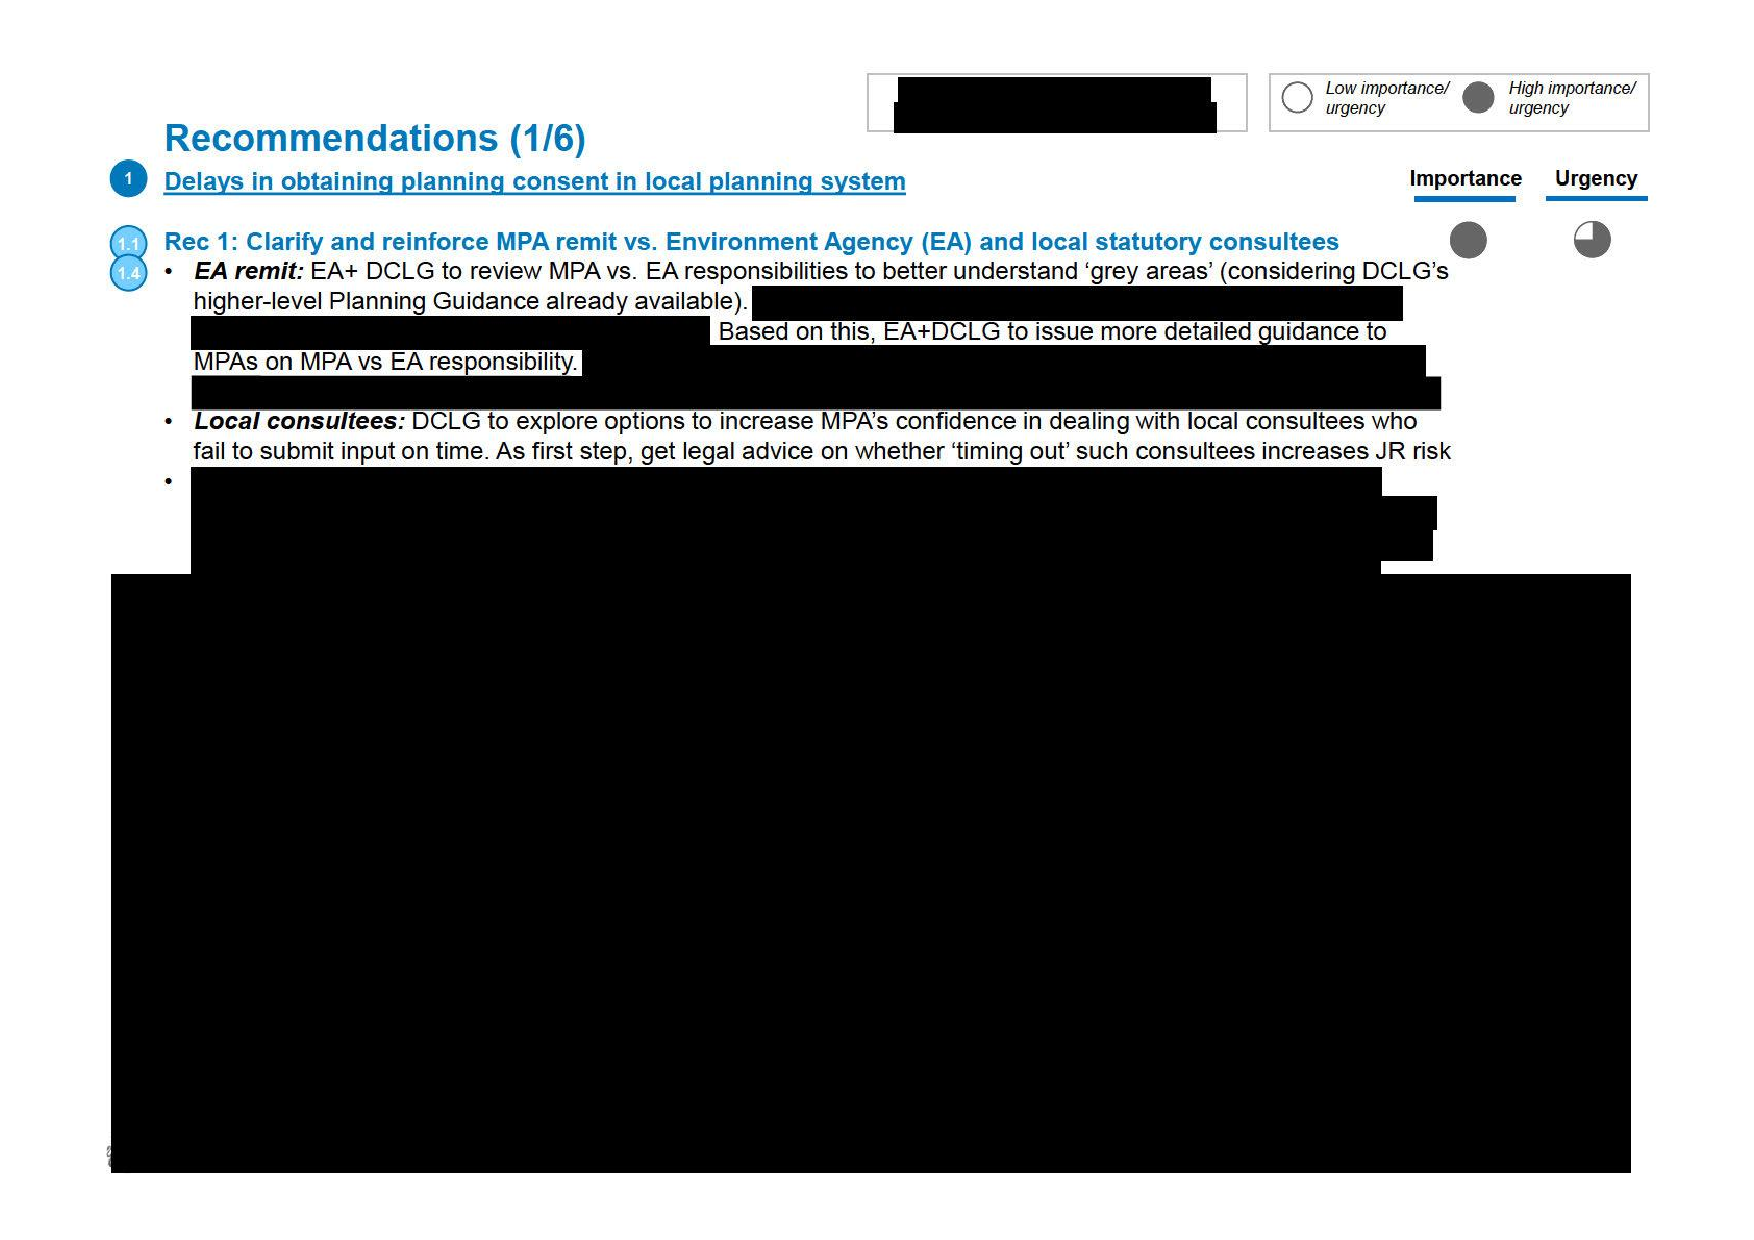
\includegraphics[width=0.6\linewidth]{figures/fracking_report_22.pdf}
    \caption{Heavily redacted excerpt from \textcite[22]{StateUKShale2016}, a report containing S41 and S43 FOIA exemptions but released in redacted form by order of \textcite{judgeshanksCabinetOfficeICO2018} following a Greenpeace FOIA request}\label{fig:fracking_report}
\end{figure}

This sensitivity review process is particularly time consuming because it has to be thorough: everything that is released has to be reviewed.
The scale of this task cannot be understated: in 2014 the total number of documents pending release stood at a staggering 817,615 records across all British government departments \autocite{allanRecordsReview2014,thenationalarchivesRecordTransferReport2014}.
Morever, this number only represents the records that have been accounted for, only within departments that keep track of these figures and must legally transfer their record to TNA.
It is safe to say that Greenwald's team's work on the Snowden archive is dwarfed in scale by the British government's Herculean backlog of records, challenging the established principle of thorough document review.

In order to preserve this paradigm, the magnitude of records calls for digital tools to accelerate the sensitivity review process.
Otherwise, the risk is for Public Institutions to become overwhelmed by their review backlog forcing them to resort to blanket closure of records for extended periods (a century), delegating the handling of sensitive information to the erosion of time and preventing rightful Public access.

\section{Objective}

Our aim is to contribute to the research into these tools to assist sensitivity reviewers with Technology Assisted Review (TAR).
Notably, we seek to extend the work in this emerging field which has produced Machine Learning classifiers focused on identifying sensitive documents to prioritize and better target reviewing resources and thus process documents faster.
A lot of effort has been dedicated to these Machine Learning algorithms, some work has focused on evaluating their impact on reducing review time, but there is little work on representing these sensitivities and displaying them in a modern user friendly interface.

We want to introduce an approach to visualizing sensitive information within documents based on these Machine Learning classifiers.
Our objective is to design, build and evaluate a proof of concept fullstack application for classifying, visualizing and redacting potentially sensitive documents.
Ideally, we aim to decrease the time reviewers spend on documents and/or allow them to more accurately identify sensitive documents.

\section{Outline}
% TODO update overview with newly added sections:
%   - Literature Review - Explanations in Machine Learning

We start with a review of the literature on the application of TAR to sensitivity review, then explore some of the works on the use of TAR in the legal profession, notably in legal discovery and finally we survey some of the research into visualization of dense information spaces.
% TODO dense information spaces might a little bullshitty?
We then evaluate similar or otherwise related products, picking out key interesting features as well as antipatterns we wish to avoid.

In order to build the application, we delineate a scope, clarifying our end product, we also establish a set of requirements to prioritize features to implement.
We elaborate on the testing methodology for our user study and lastly we draw up wireframe diagrams to have a draft layout of components in the application and to get a better sense of feature priorities

We then discuss our application design process. We elaborate on our choice of technologies, the reasons for our final choice as well alternative options and why we did not choose them. We ultimately summarize our technology stack.

We detail some of the key pieces of software, highlight key sections of the code as well as our Repository and Continuous Integration setup.
We explain the issues we ran into, from data storage concerns to frontend implementation struggles as well as Machine Learning classifier optimization and debugging.

Lastly before concluding, we detail the findings from an evaluation by an expert panel, as well as the user evaluation we would have conducted had the COVID-19 pandemic not rendered it infeasible.


%==================================================================================================================================
\chapter{Background}

\section{Literature Review}

\subsection{Technology Assisted Sensitivity Review}

\autocite{sanchezDetectingSensitiveInformation2012}

Research into the application of TAR to sensitivity review began with \textcite{mcdonaldClassifierDigitalSensitivity2014} which established an initial Machine Learning sensitivity classifier.
They combined the textual content of sensitive documents with sentiment analysis, a custom country risk score, entity and name recognition and achieved a balanced accuracy (BAC) of 0.63 for FOIA S27 and 0.74 for S40.

\textcite{berardiSemiAutomatedTextClassification2015} establishes that BAC and the \(F_{2}\) measure are best suited when evaluating sensitivity classifiers due to the predominance of recall over precision: a released sensitive document is potentially more problematic than an excessive closure of information.
As such, rather than an automated \textit{replacement}, they frame the solution as an \textit{aid} to sensitivity reviewers.
They demonstrate the advantage of a utility-theoric approach to maximizing reviewer effectiveness.
Specifically they focus on the human reviewer validation of the automated classifier's labelling: prioritizing the review document with a high probability of an ``automated misclassification''.

\textcite{mcdonaldUsingPartofSpeechNgrams2015} expanded on the idea and improved classification with Part-of-Speech tagging of large N-grams filtering out those which are not characteristic of a sensitive document by calculating n-grams' ``sensitivity load'' \autocite[2]{mcdonaldUsingPartofSpeechNgrams2015}.
This results in 0.73 balanced accuracy and 0.51 \(F_{2}\) when identifying a subset of S27 FOIA exemptions: ``information supplied in confidence''.

This work was furthered with an in depth study of SVM kernel functions' performance for POS sequence classification \autocite{mcdonaldStudySVMKernel2017}.
The paper also combined the POS sequence classification with full text classification to obtain a maximum \(F_{2}\) measure of 0.46 and a maximum BAC of 0.64 for S27 and S40 sensitive documents combined.
\autocite{mcdonaldEnhancingSensitivityClassification2017} further expand this model on the same dataset, obtaining a BAC of 0.71 and \(F_{2}\) of 0.54 using Word embeddings and semantic features.

\textcite{mcdonaldActiveLearningStrategies2018} implement ``Active Learning'' of reviewer annotations for dynamically prioritizing documents in a collection in order to maximize the automated classifier's effectiveness with the least possible manually review docuements.
They achieve a BAC of 0.7 on the same collection as \textcite{mcdonaldStudySVMKernel2017,mcdonaldEnhancingSensitivityClassification2017} but with a 51\% reduction in the number of manually reviewed documents.

\textcite{mcdonaldHowSensitivityClassification2019} conduct a user study to evaluate the impact of classification effectiveness on reviewers' performance. With the aid of a simple interface, they asked reviewers to identify S27 and S40 FOIA sensitivities with and without sensitivity classifier predictions.
They conclude that, while participants' identified sensitivities were randomly correct, they however find a BAC between 0.69 and 0.8 for participants aided respectively with medium and perfect classifier prediction performance.

\subsection{``Predictive Coding'' or \textit{TAR} for legal electronic discovery}

Ongoing research in the area of Judicial practice has applied the concept of TAR to the process of legal discovery.
This research has coined the term ``Predictive Coding'' \autocite{carrollGrossmancormackGlossaryTechnologyassisted2013} as an industry specific use of TAR in the legal practice, particularly for ``legal discovery'', the pre-trial exchange of evidence by both parties.
Parallels can be drawn with the task of sensitivity review, specifically the process of identifying ``privileged information'' in a legal discovery corpus.
% TODO elaborate on privilege (both attorney-client and common interest)

\textcite{grossmanTechnologyAssistedReviewEDiscovery2010} compared the performances of a manual and TAR aided eDiscovery process with data from the various teams of the TREC 2009 Legal Track \autocite{hedinOverviewTREC2009}.
They conclude that TAR methods lead to more accurate eDiscovery relevance estimations with significantly lower effort than with an exhaustive manual discovery process.

One of these teams, \textcite{cormackMachineLearningInformation2009}, constructed various training sets for a given list of discovery topics from a corpus of eDiscovery documents using IR techniques (a search engine).
They then fitted Logistic regression classifiers on these training sets to classify the rest of the collection as relevant or not for each topic.
Ultimately, this team obtained the best F1 measure averaged across all topics \autocite{hedinOverviewTREC2009}.
Moreover, ``by all measures, the average efficiency and effectiveness of the five technology-assisted reviews surpasses that of the five manual reviews'' \autocite[p.~43]{grossmanTechnologyAssistedReviewEDiscovery2010}.

The task at hand is different from the sensitivity review of sensitive documents.
Firstly, the implications of missing a relevant document in sensitivity review can be far greater than in legal discovery.
The works we have cited above only manually reviewed fractions of their document collection, accepting a level of ``misclassification'' that is not tolerable in sensitivity review.
% TODO Source this in the works of the Macdonalds
Indeed, even with reliable classifiers, all documents will need to be manually reviewed for sensitivities.
The task of identifying ``privileged'' information in legal discovery documents is the one that comes closest that of sensitivity review.

\section{Explanations in Machine Learning}


\autocite{ribeiroWhyShouldTrust2016}

\autocite{lundbergUnifiedApproachInterpreting2017}

\section{Approaches to document visualization}

\subsection{Lexical Episode Plots}
%
\begin{wrapfigure}{r}{0.4\textwidth}
    \centering
    \begin{subfigure}[c]{0.2\textwidth}
        \centering
        \small
        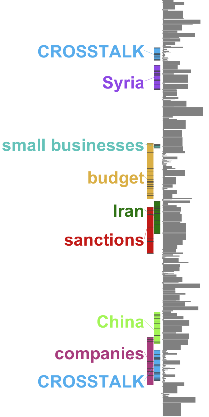
\includegraphics[width=\linewidth]{images/document_visualization/topic-overview.png}
        \caption{Lexical Episode Plots}\label{fig:lexical_plot}
    \end{subfigure}
    \hspace{0.01\textwidth}
    \begin{subfigure}[c]{0.17\textwidth}
        \centering
        \small
        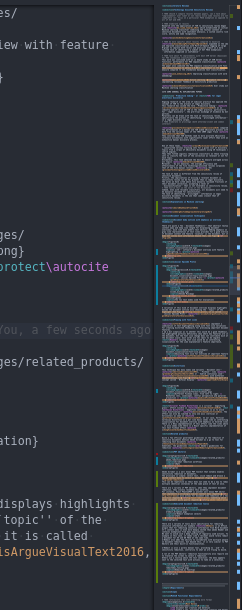
\includegraphics[width=\linewidth]{images/related_products/vscode_minimap.png}
        \caption{VSCode Minimap}\label{fig:vscode_minimap}
    \end{subfigure}
    \caption{Document Overviews}\label{fig:test-modes}
    \vspace{-40pt}
\end{wrapfigure}

A variation of this kind of document overview displays highlights beside the document outline also showing the ``topic'' of the highlight (Figure~\ref{fig:lexical_plot}), it is called ``Lexical Episode Plots'' \autocite{el-assadyVisArgueVisualText2016,goldExploratoryTextAnalysis2015}.

It is reminiscent of code overviews in text editors, especially those aimed at editing code, which provide an overview of the ``shape'' of the text with syntax highlighting colour to allow fast navigation between sections of source code like what \textcite{MicrosoftVscode2020} implements (Figure~\ref{fig:vscode_minimap}).

An old Information Retrieval system, J24 \autocite[7]{ogdenDocumentThumbnailVisualizations1998}, implements a similar feature, highlighting query terms in a document outline
This shows that perhaps, these sort of overviews could also be used before viewing a document, as a popup view when a document is hovered on within a collection.

\subsection{Varying font size}

\begin{wrapfigure}{l}{0.4\textwidth}
    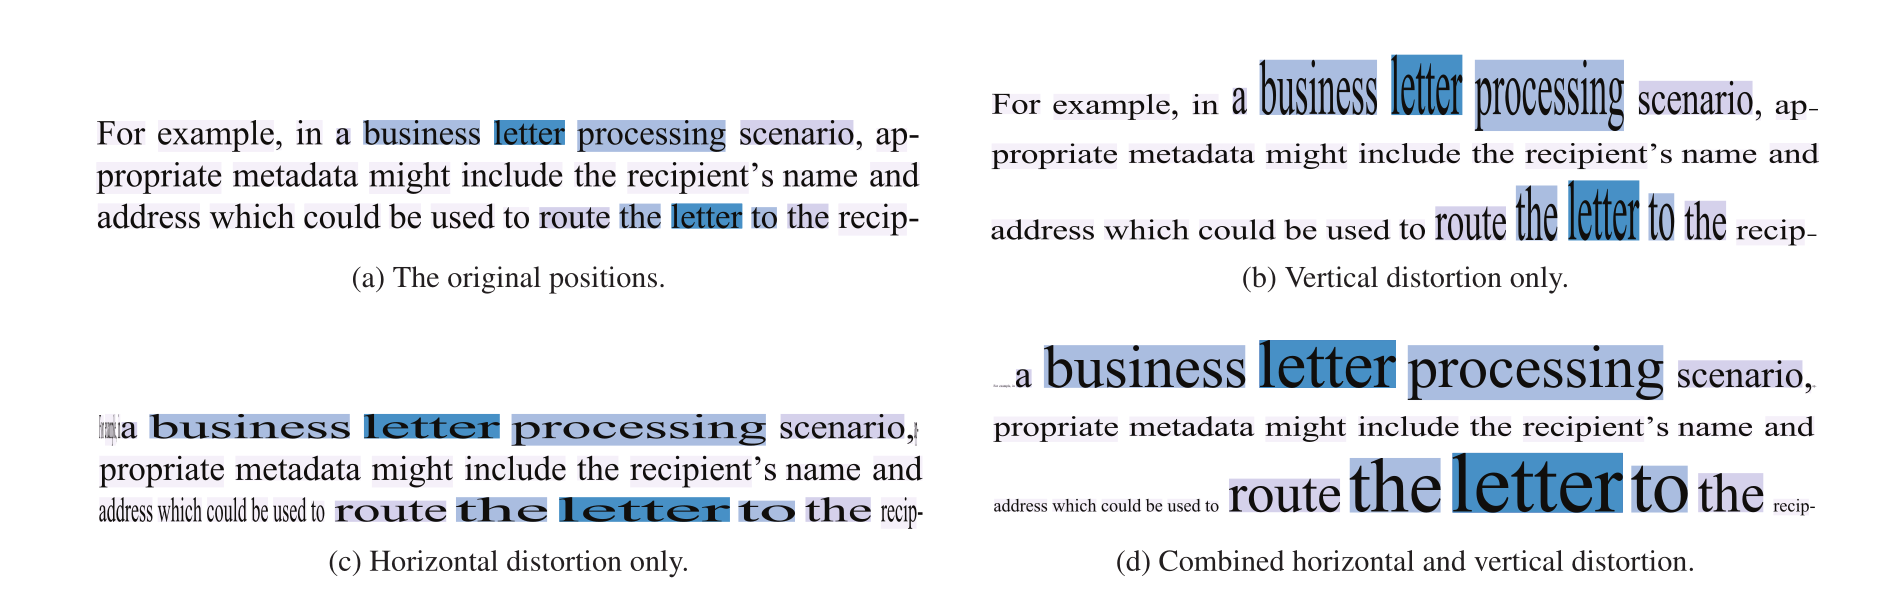
\includegraphics[width=\linewidth]{images/document_visualization/font-size.png}
    \caption{Adjusting font size}\label{fig:font-size}
    \vspace{-10pt}
\end{wrapfigure}

\textcite{stoffelDocumentThumbnailsVariable2012} implement a combination of text highlighting along with font size variations for creating distorted thumbnails for previewing important document features (Figure~\ref{fig:font-size}).
It is not certain this would be a good thumbnail, the highlighted portions definitely show where key features are in the document, but a lot of the document structure is lost.
However varying font size within a \textit{reasonable range} would be an interesting visualization for the visualizing feature importance in a prediction.

\subsection{Distortion}

This technique has many names and variants ``Document Lens'' \autocite{robertsonDocumentLens1993}, ``Fisheye'' view \autocite{greenbergFisheyeTextEditor1996} or ``hybrid continuous zoom'' \autocite{bartramContinuousZoomConstrained1995} with different implementations (see Figure~\ref{fig:fisheyes}) they are part of a concept called ``Bifocal Display'' \autocite{apperleyBifocalDisplay}.

\begin{figure}[H]
    \centering
    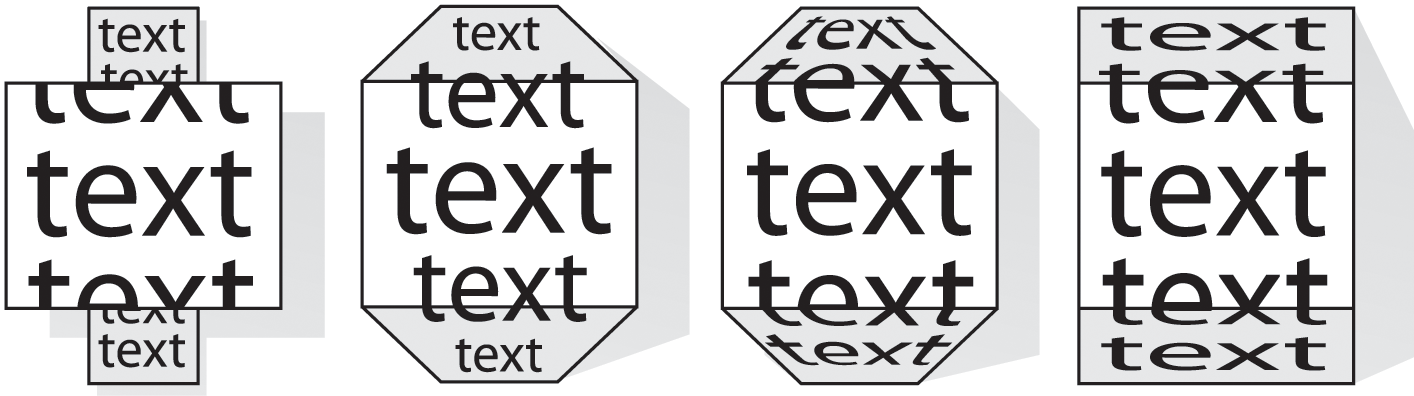
\includegraphics[width=0.6\textwidth]{images/document_visualization/different-fisheyes.png}
    \caption{Fisheye views, from left to right: \\
        Manhattan lens, zoomscapes, central perspective and parallel projection \\
        \protect\autocite{baudischFishnetFisheyeWeb2004}
    }\label{fig:fisheyes}
\end{figure}

\textit{Circular Fisheye Distortion} is a circular ``magnifying glass'' effect visible in \textcite{bostockFisheyeGrid2019}. \textit{Cartesian Distortion} ``magnifies continuously so as to avoid local minification'' \autocite{bostockFisheyeDistortion2012}. The effect can also be limited to only one axis (vertical or horizontal) as seen in \textcite{pstuffaCartesianFisheyeDistortion2019}. In our case, Vertical Cartesian Distortion on a per line basis seems like an interesting visualization for document overview with emphasis on hovered lines. There is a D3js implementation of this effect \autocite{pstuffaCartesianFisheyeDistortion2019}, it also seems like there is a React specific implementation of this text fisheye effect \autocite{zhongVincentdchanReactfisheye2019}.

\section{Related products}

\subsection{PDF editors}

Quite a few official government guidelines on the redaction of sensitive documents mention Adobe Acrobat as a go to tool for redacting text documents \autocite{thenationalarchivesRedactionToolkitPaper2016}.
Sometimes, the guidelines \textit{are} Adobe's guidelines for redaction \autocite{scottishgovernmentRedactingInformation2019}.

\begin{wrapfigure}{r}{0.5\textwidth}
    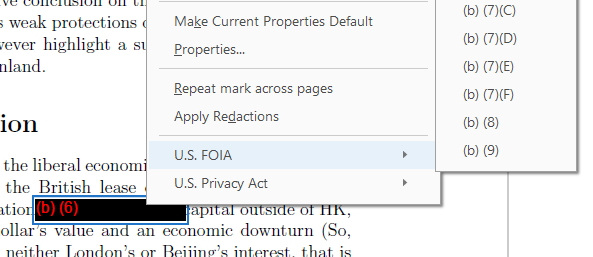
\includegraphics[width=\linewidth]{images/related_products/adobe_redaction.png}
    \caption{Acrobat redaction workflow}\label{fig:adobe-redaction}
    \vspace{-20pt}
\end{wrapfigure}

Adobe Acrobat is a well known PDF toolkit that notably enables sensitivity redaction of documents.
The principle is simple: select text, click redact and browse a nested context menu to select an exemption (Figure~\ref{fig:adobe-redaction}).
This can be repetitive as their does not seem to be a way to redact multiple identical instances of the same piece of text at once.

There are a variety of PDF editors, when they implement document redaction, they closely resemble this workflow.
For instance, Foxit PhantomPDF is another well known PDF editor that implements a strikingly similar context menu (Appendix~\ref{fig:foxit-menu}) also allows for document wide redaction of a text selection (Appendix~\ref{fig:foxit-redact-all}), something which Adobe implement quite poorly (Appendix~\ref{fig:adobe-redact-all}).

\subsection{Dedicated document redaction tools}

\begin{wrapfigure}{l}{0.4\textwidth}
    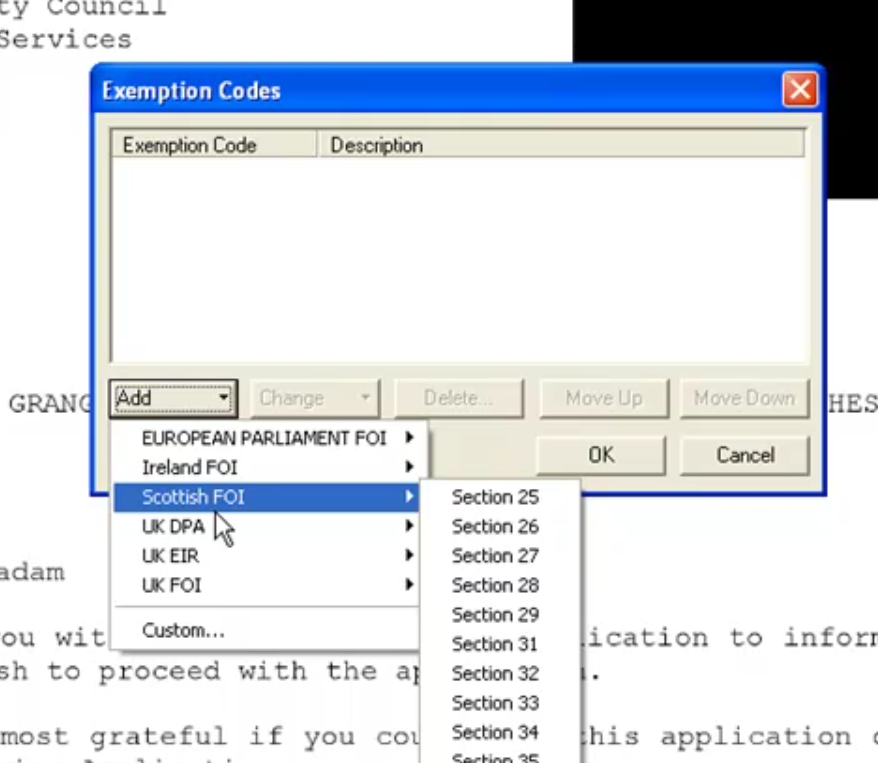
\includegraphics[width=\linewidth]{images/related_products/eredact_dropdown.png}
    \caption{e-Redact exemption selection}\label{fig:eredact-dropdown}
    \vspace{-17pt}
\end{wrapfigure}

There are a few tools built specifically for redacting sensitive information,for example \textcite{ERedact} is a Microsoft Office plugin that for redacting sensitive information from documents.
It's context menu is even more deeply nested than Adobe Reader's and contains exemptions from many legislations (Figure~\ref{fig:eredact-dropdown}).
We want to avoid such a deep nesting of regularly used actions, for example in this case, it seems like a reviewer would rarely redact a document for US and UK FOIA at the same time.
A solution to this would be to have a setting to select the legal ``framework'' within a settings menu which would reduce deep menu nesting.
e-Redact also adds the ability to collaborate with multiple people on document redactions, but beyond this, it is very similar to PDF Editors and their built-in functionalities.

\textcite{ERedact} is also a purely manual tool, providing no ``aid'' to sensitivity redaction, contrarily to what we are trying to build.

A lot of the PDF editors' redaction functionality also require one to traverse the screen to select a redaction.

Others such as \textcite{RedactedAIRemovea} use a tooltip above the text selection (albeit not consistently): the menu appears next to the selected text with actions to take on a selection which avoids having to cross long screen distances (Figure~\ref{fig:redactedai}).
A downside of their implementation of a ``popup menu'' is that it takes considerable space, while it does offer quite a few useful actions, its ``remove'' and ``unredact this'' button are quite large,, we prefer a smaller menu that hides less of the content.

In fact, \textcite{RedactedAIRemovea} is a similar concept to what we are trying to achieve: it is a web application for redacting sensitive documents. Its flagship feature uses Natural Language Processing (NLP) methods (namely: entity extraction) to provide an aid to document reviewers (Figure~\ref{fig:redactedai}).

\begin{figure}[H]
    \centering
    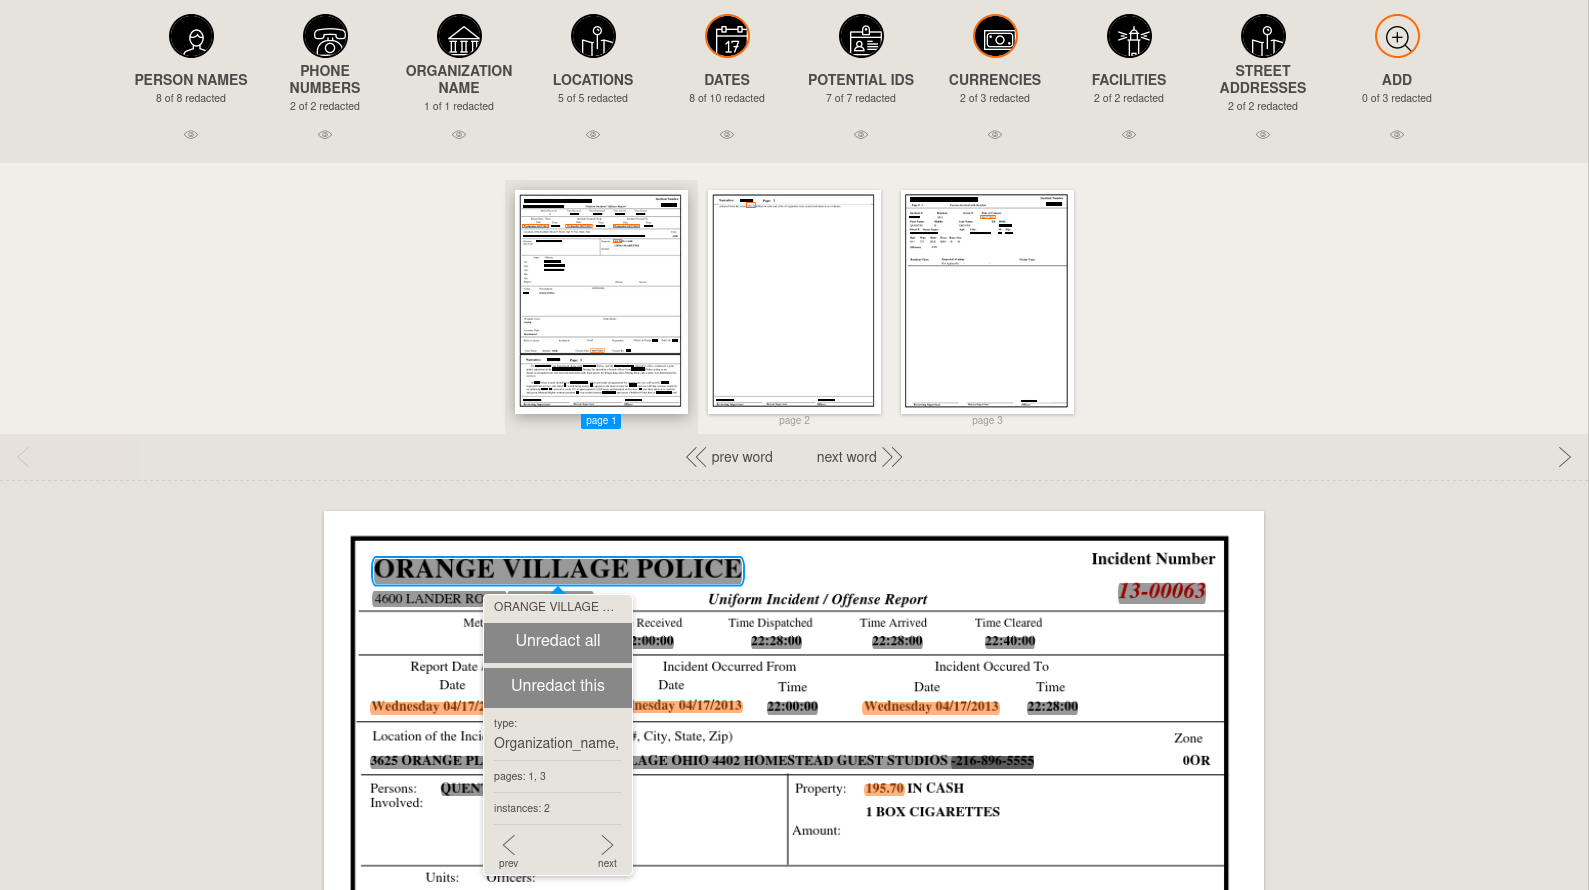
\includegraphics[width=0.95\linewidth]{images/related_products/redactedai.png}
    \caption{Redacted.ai document view}\label{fig:redactedai}
\end{figure}

%==================================================================================================================================
\chapter{Requirements}

\section{MoSCoW Functional Requirements}

% TODO reformulate this into something more formal
\begin{adjustbox}{width=\textwidth,center}
    \begin{minipage}[t]{.5\linewidth}
        \centerline{\textbf{Must Have}}
        \begin{enumerate}[label=\textbf{M\arabic*}]
            \item Document Set creation and deletion
            \item Within a set, plaintext document creation and deletion
            \item Predicted document sensitivity classification (sensitive or not?)
            \item Explanation for aforementioned classifications
            \item User classification of a document (sensitive or not?)
            \item Document set statistics (number of sensitive documents etc\ldots)
            \item Document sets order documents by sensitivity
            \item User redactions of a document with text highlighting, with possible edits and save functionality
            \item Final redacted document exporting
            \item Documentation for API
        \end{enumerate}
    \end{minipage}
    \hfill
    \noindent
    \begin{minipage}[t]{.5\linewidth}
        \centerline{\textbf{Should Have}}
        \begin{enumerate}[label=\textbf{S\arabic*}]
            \item User redactions helper (highlight all instances of redacted text, could do this on a document set level)
            \item For a document, suggest redaction of sensitive elements
            \item Fulltext document search
        \end{enumerate}
    \end{minipage}
\end{adjustbox}

\vspace{0.5cm}

\begin{adjustbox}{width=\textwidth,center}
    \begin{minipage}[t]{.5\linewidth}
        \centerline{\textbf{Could Have}}
        \begin{enumerate}[label=\textbf{C\arabic*}]
            \item Extract and display entities from document
            \item Possibility of using different text Classifiers
            \item Documentation for API SDK
            \item Documentation for frontend
            \item Reviewer authentication
        \end{enumerate}
    \end{minipage}
    \hfill
    \noindent
    \begin{minipage}[t]{.5\linewidth}
        \centerline{\textbf{Would Have}}
        \begin{enumerate}[label=\textbf{W\arabic*}]
            \item Handle more than plain text files (PDF, Word etc…)
            \item Specified and enforced document size and count upload limits
            \item ``Active Learning'': user redactions help improve future predictions
            \item Deployed ``production'' web application
        \end{enumerate}
    \end{minipage}
\end{adjustbox}
\section{Scope and non-functional definition}

We should reiterate that our objective is not to have a ``production ready'' deployable application.
Rather the emphasis is on producing a proof of concept application to experiment with sensitive document visualizations.
As such, we de-prioritized features like reviewer authentication and having a deployable application.

We aim to bring a ``modern looking'' interface, tools like PDF editors or the Office plugin we saw provide an ageing interface often with excess complexity.
We think that an approach with correctly applied modern design guidelines such as Google's \textcite{MaterialDesign} improves user experience, both in terms of aesthetics and usability.

Originally, we set out to focus on both document set visualization as well as single document visualization, ultimately however the focus shifted a lot towards the document viewer.

As mentioned we include a user study within the scope of this study to evaluate our application.

\section{Wireframing}

\begin{figure}[H]
    \centering
    \begin{subfigure}[b]{\linewidth}
        \centering
        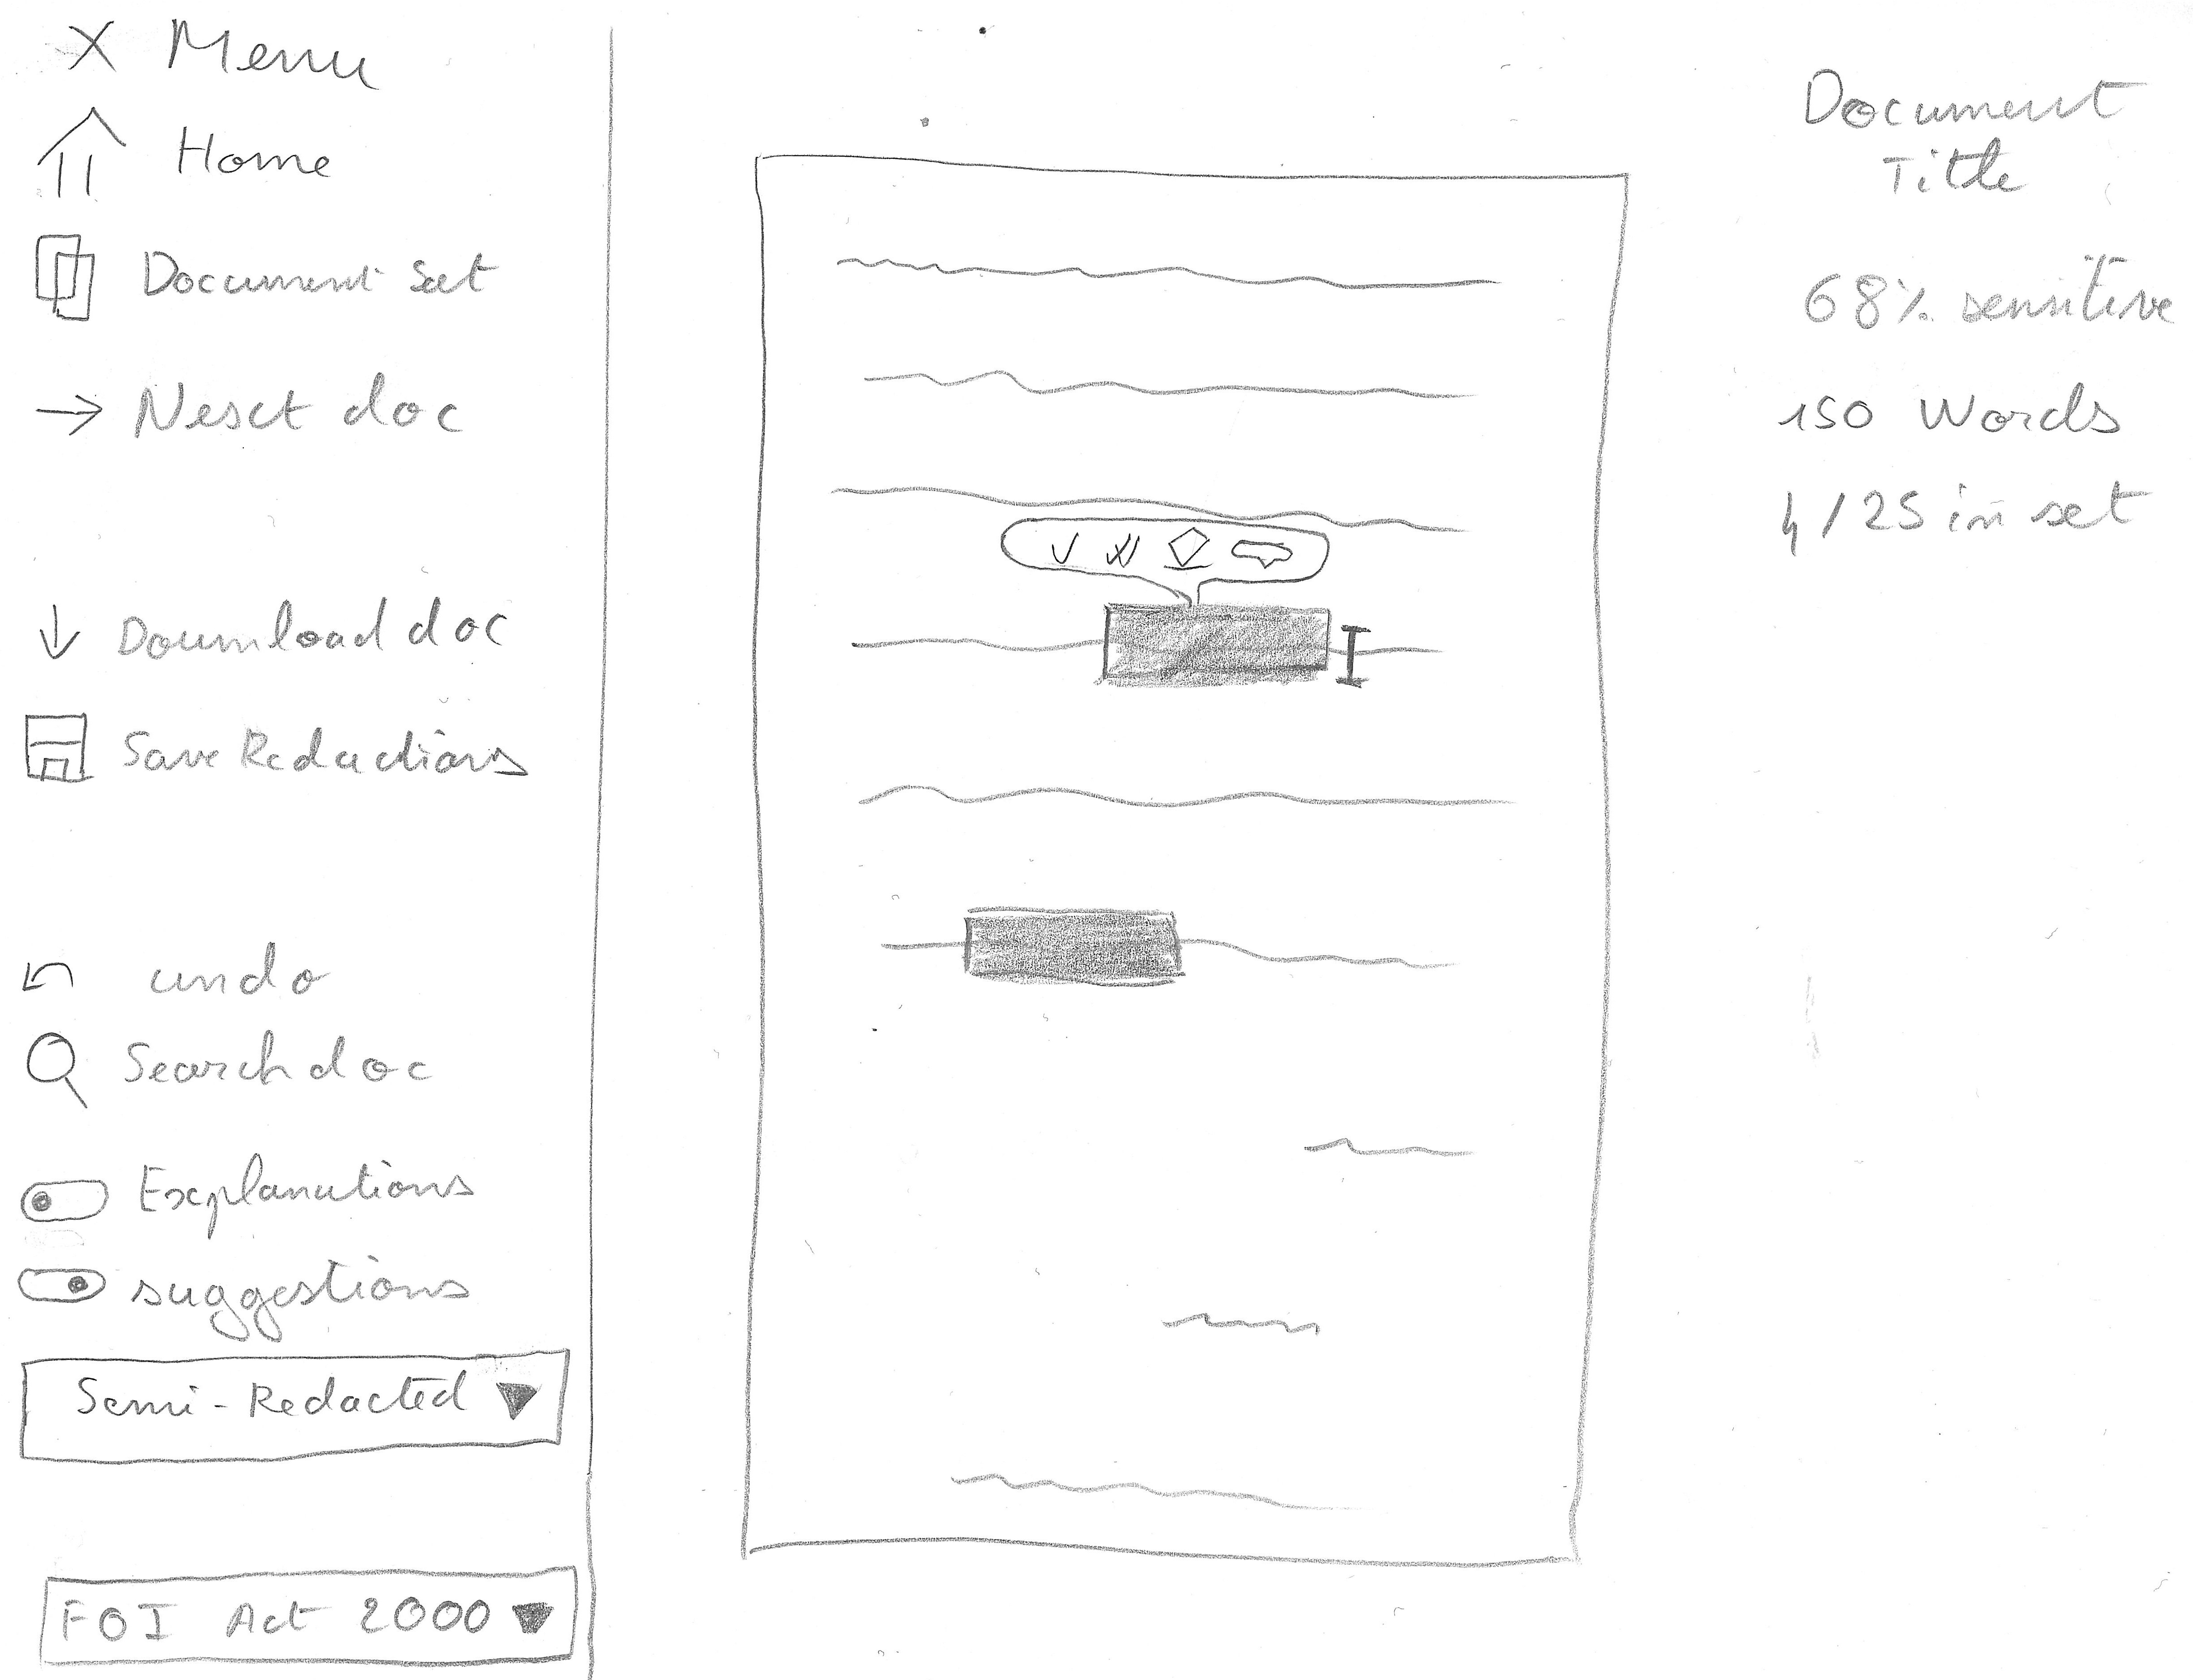
\includegraphics[width=0.6\linewidth]{images/wireframes/doc_view.jpg}
        \caption{Document View Wireframe}\label{fig:document-wireframe}
    \end{subfigure}
    \begin{subfigure}[b]{\linewidth}
        \begin{subfigure}[b]{0.5\linewidth}
            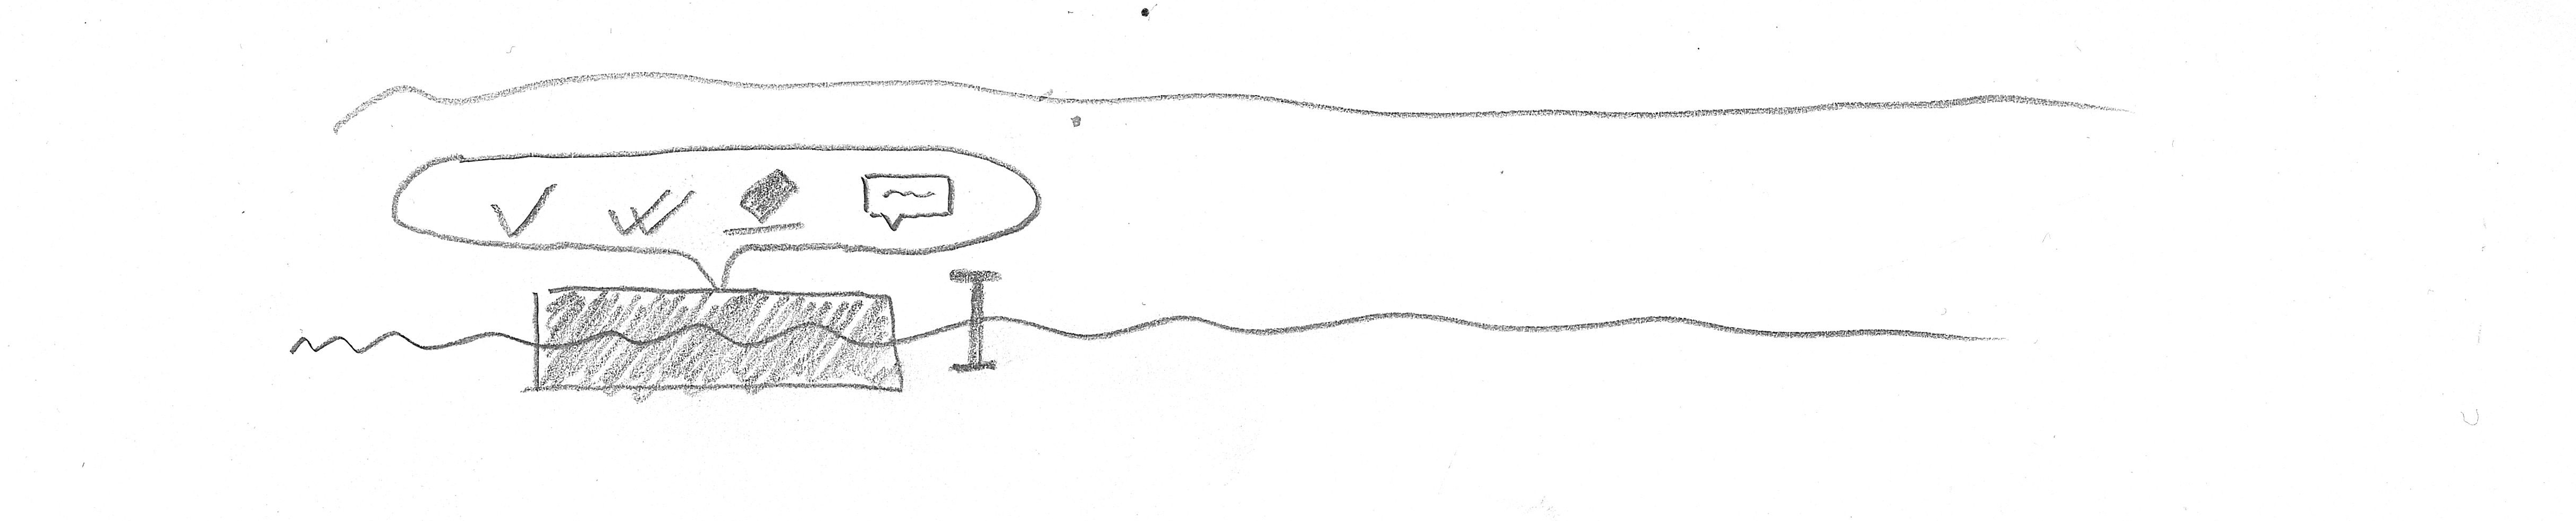
\includegraphics[width=\linewidth]{images/wireframes/tooltip.jpg}
            \caption{minimized tooltip wireframe}\label{fig:tooltip-wireframe}
        \end{subfigure}
        \begin{subfigure}[b]{0.4\linewidth}
            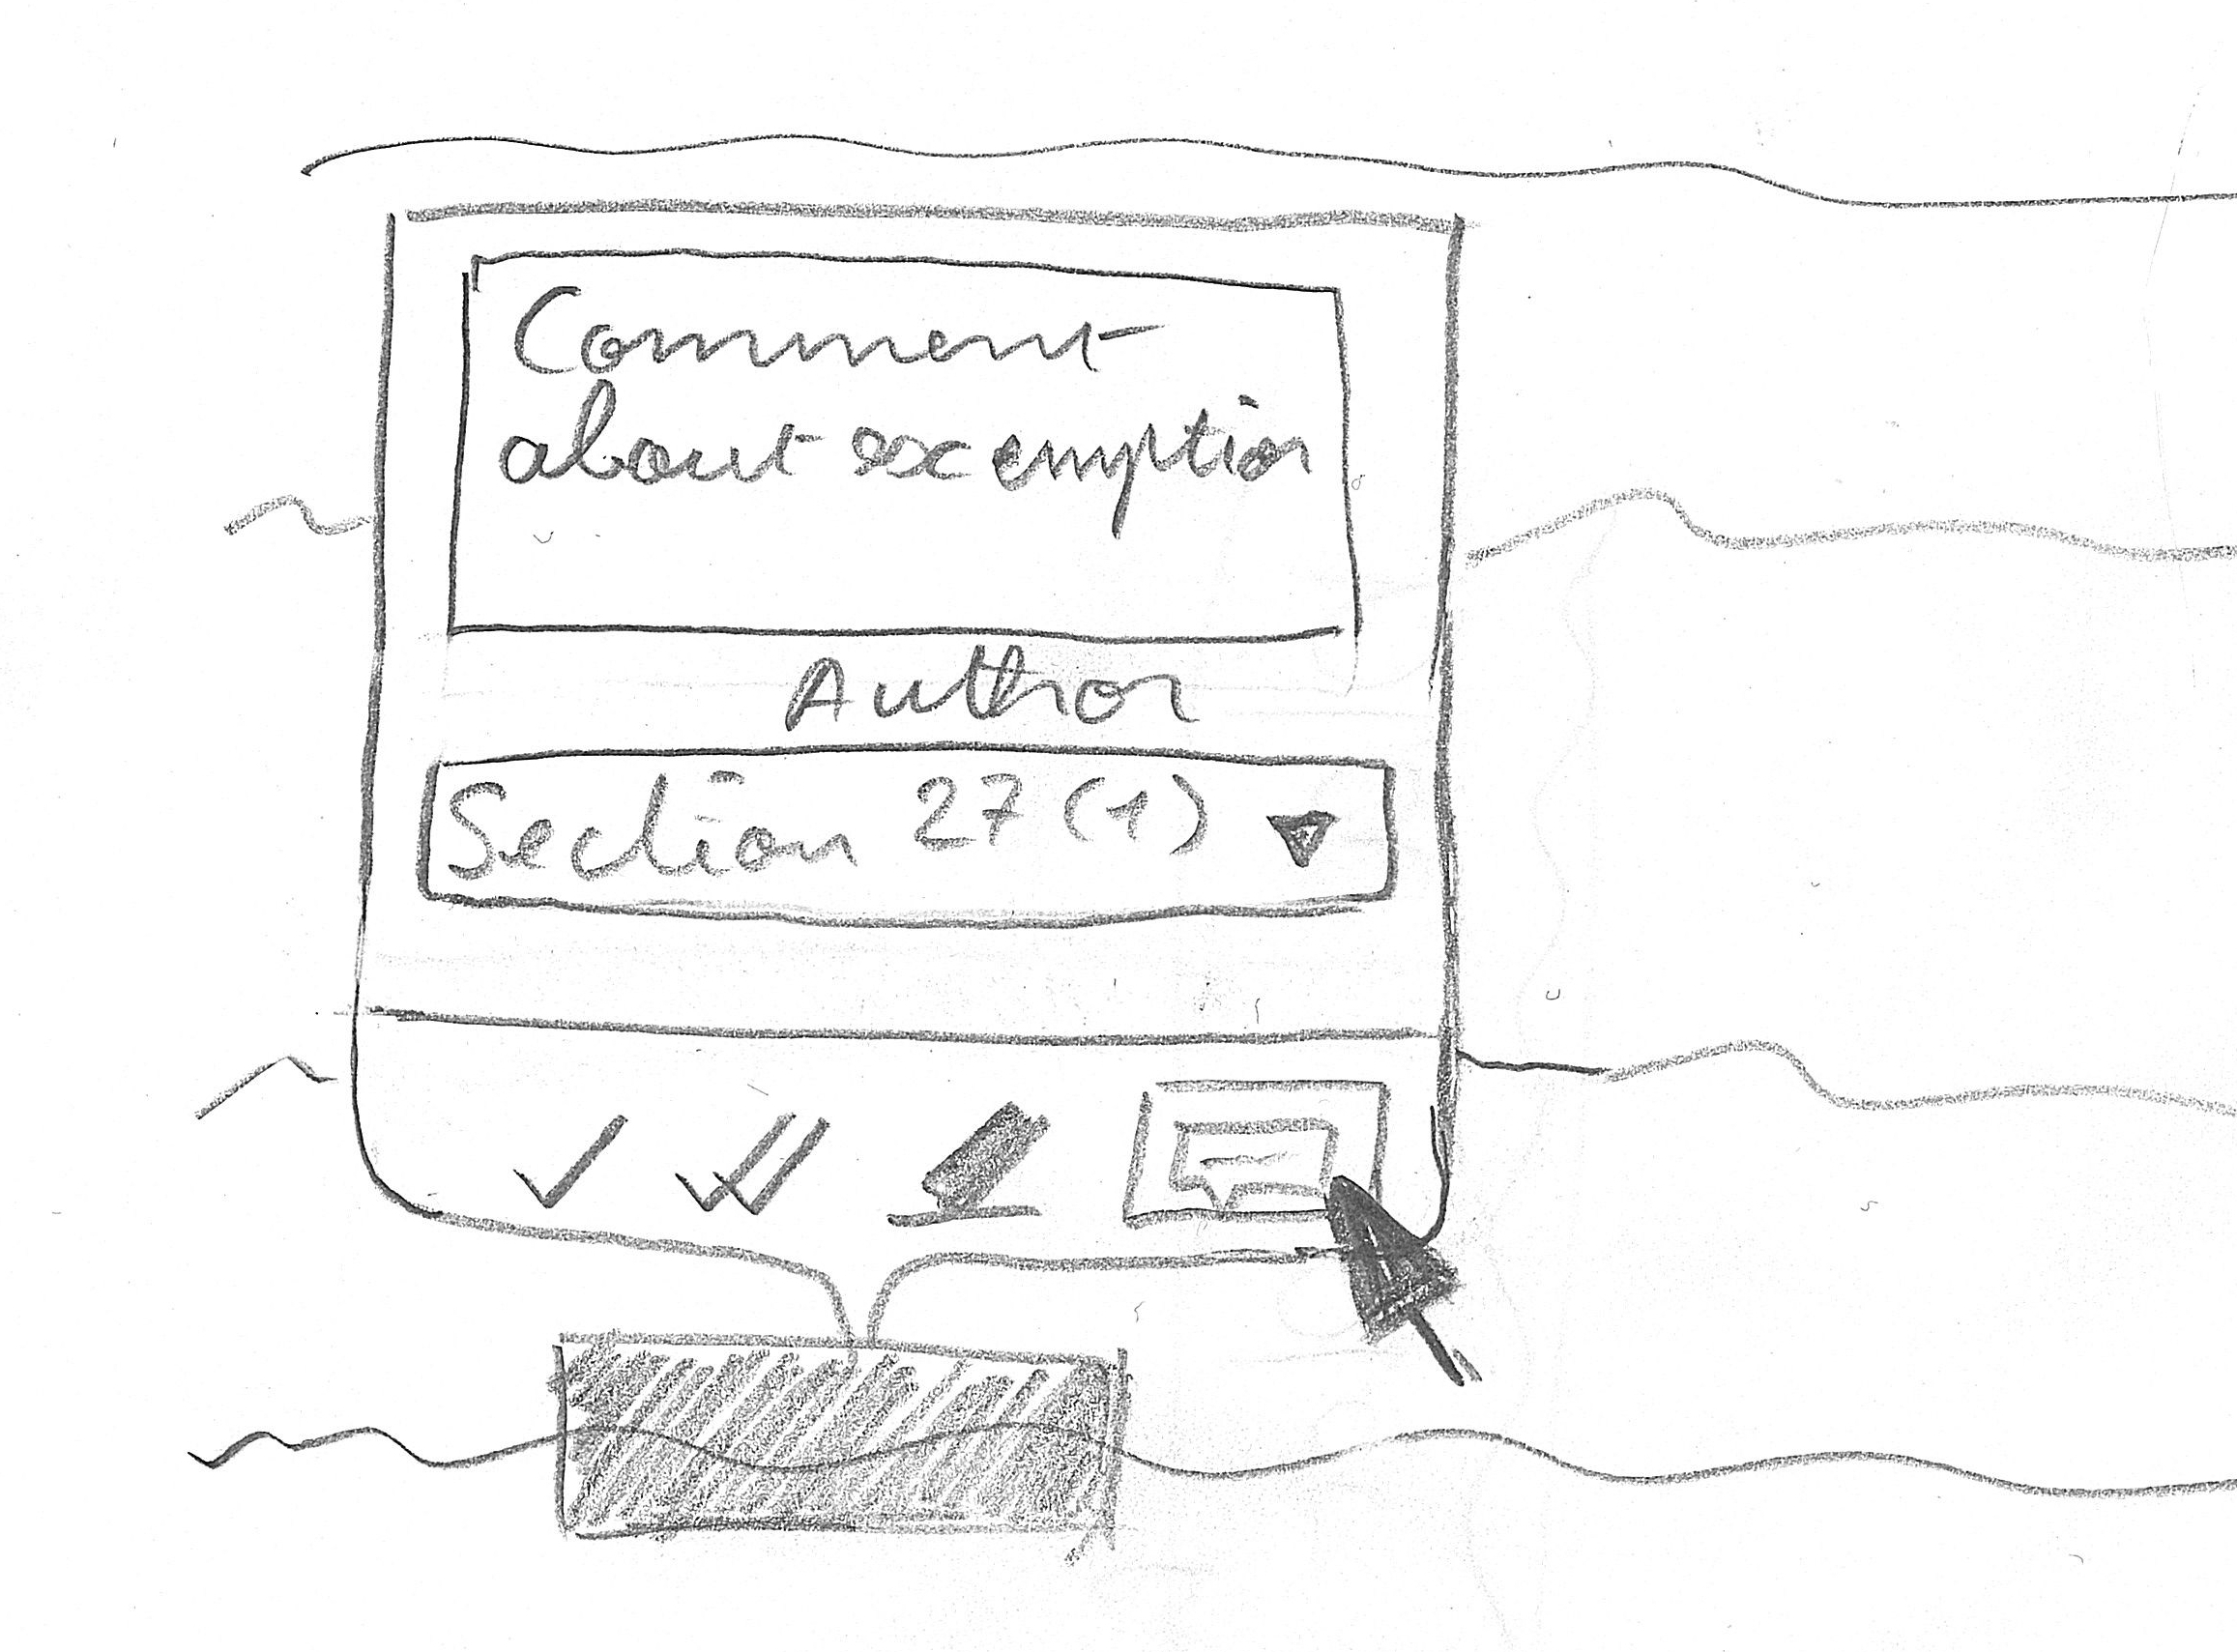
\includegraphics[width=\linewidth]{images/wireframes/tooltip_comment.jpg}
            \caption{Expanded tooltip wireframe}\label{fig:expanded-tooltip-wireframe}
        \end{subfigure}
    \end{subfigure}
    \caption{Selection of some of the Wireframes drawn up during the design process}\label{fig:wireframes}

\end{figure}


%==================================================================================================================================
\chapter{Design}

% link back to requirements
% choice of technologies

\section{Application structure}

\begin{figure}[H]
    \centering
    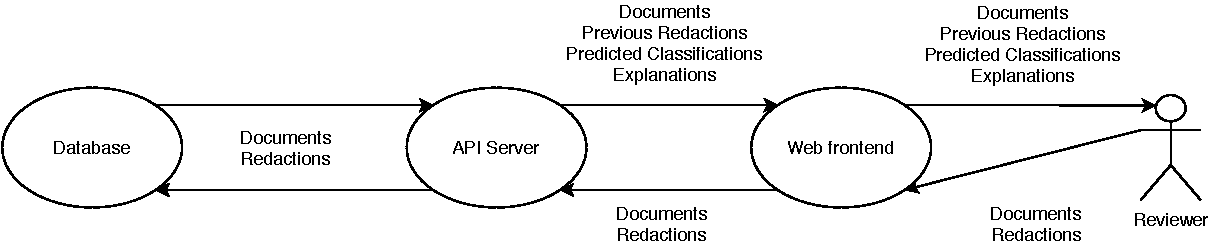
\includegraphics[width=\textwidth]{figures/design_diagram.pdf}
    \caption{Application Structure and information flow}\label{fig:design_diagram}
\end{figure}

\section{Machine Learning Model and explanations}

% TODO this sounds too much like a list
% TODO justify choice of ML library
We use the Scikit-Learn library to implement our Machine Learning Models \autocite{pedregosaScikitlearnMachineLearning2011} for predicting the sensitiity of documents to meet requirement \textbf{M3}, \textbf{M7} and \textbf{M6}. For performance reasons, we replaced its SVC implementation with a drop-in parallel replacement ``ThunderSVM'' which can operate on multicore CPUs or CUDA enabled GPUs \autocite{wenThunderSVMFastSVM2018}.

We satisfy our requirement \textbf{M4} for explanations and more generally better understanding of our classifier's predictions using techniques implemented by the Lime library \autocite{ribeiroWhyShouldTrust2016} which provides per-feature weights explaining the feature's contribution to the final classification.

\section{OpenAPI specification and generator}

``The OpenAPI Specification is a community-driven open specification within the OpenAPI Initiative, a Linux Foundation Collaborative Project.'' \autocite{OAIOpenAPISpecification2020}.
% TODO elaborate a bit more on this
It is an increasingly popular framework for formally defining a REST API contract.
Its precision and specificity is such that it has allowed powerful tools to expand it.
Notably, the OpenAPI generator \autocite{OpenAPIToolsOpenapigenerator2020} which, given an OpenAPI specification, allows for the \textit{automatic} generation of API server code in more than 40 languages and API client code in more than 50.
Hence, we chose to write our API specification in OpenAPI format \textit{before} developing the API.
This allowed us to generate boilerplate API server and client code with documentation simply given the precise documentation thus fulfilling requirements \textbf{C3} and \textbf{M10}.

\section{API Server}

Most of our data science tools are written in Python which is why we selected it to write our API server.
Furthermore, the language's broad library selection makes development easier, notably for implementing requirements such as \textbf{W1} and \textbf{C5}
The question of the choice of framework, remained, specifically since the OpenAPI generator allows for the generation of Python Server code with different frameworks.

We chose the implementation that makes use of an OpenAPI wrapper around Flask called Connexion which handles ``the mapping from the specification to the code.
This incentivizes you to write the specification'' \autocite{ZalandoConnexion2020}.
Furthermore, Flask is a Python API framework that is extensible with libraries notably implementing file upload size limits for requirement \textbf{W2}. Furthemore it is widely used by major technology companies like Reddit or Netflix \autocite{WhyDevelopersFlask}, a testament to its robustness and level of support which streamlines the implementation of requirement \textbf{M9}.

Furthermore, the Connexion+Flask implements the Oauth2 Authentication specification for API endpoints, a state of the art authentication framework that allows us to securely authenticate reviewers for requirements \textbf{C5} \autocite{jonesOAuthAuthorizationFramework2012}.

\section{Frontend}

We chose to implement a web application as the frontend for our application.
This allows for compatibility with many devices: generally anything that can run a reasonably modern web browser can use a web application without worrying about Operating System choice or GUI library compatibility.
We identified early on the need for a ``dynamic'' application meaning that in order to implement a web application, the codebase would be prominently Javascript (JS).

There are a number of modern frameworks that facilitate JS web application development and avoid having to write plain JS.
Their ``component'' approach to UI elements allows for the development of standalone modules that can be combined into an application, streamlining development by relying on high quality component libraries such as \textcite{Materialui2020} or visualization plotting libraries like \textcite{Recharts2020}.
There are three major web JS frameworks: \textcite{Angular2020,FacebookReact2020,VuejsVue2020}.

Angular is a web framework developed by Google, development uses TypeScript (TS) which is a type language that can transcompile into Javascript.
It has a strict separation of styles (CSS), markup (HTML) and function (TS) and is generally much more ``opinionated'' on application structure and development.
These ``restrictions'' can, at the scale of large projects become standards enabling more streamlined collaboration, at our scale however (one developer), we viewed them as more of a hindrance than an enablement especially since our scope is that of a \textit{Proof of Concept} more than a final large scale project \autocite{wohlgethanSupportingWebDevelopmentDecisions2018}.

VueJS holds similar ``opinions'' on project structure but encapsulates all aspects of a component into a \lstinline{.vue} file albeit while being more ``liberal'' than Angular (by externalizing State management and routing for example) \autocite{wohlgethanSupportingWebDevelopmentDecisions2018}.
Furthermore, like Angular, VueJS introduces a special syntax for enhancing the templates with \lstinline{for} loops and \lstinline{if} statements.

Perhaps the ``most flexible'' framework is ReactJS which we chose as our frontend framework.
ReactJS uses \lstinline{.jsx} files which allow for the integration of HTML and CSS within JS, which avoids the custom syntax used by Angular and VueJS and allows for the versatile use of JS for introducing logic into templates.
Furthermore ReactJS is an Open Source project developed by Facebook, this backing along with its flexibility has given birth to a large ecosystem of both development support and advanced component libraries \autocite{wohlgethanSupportingWebDevelopmentDecisions2018}.
It does however introduce more complex state management due to its ``one-way data binding'': information flows from parent to child component but the reverse operation needs to be done through callbacks or using a state management libraries like \textcite{Redux2020}.
These problems mostly become prominent on larger scale projects, hence we opted for the flexibility of ReactJS for a quickly starting development, albeit encountering some of these state management issues in the latter stages of the project.
% TODO refer back to proof of concept scope of project to justify this

\section{Packaging application components}

We chose to package all these services as \textcite{Docker2020} containers.
Docker is a high level container-based virtualization tool.
A docker container performs better than a Virtual Machine (VM) as it runs on the host's kernel while also providing a good level of isolation from the host through namespaces and cgroups.
Most importantly, the docker ecosystem is much evolved than alternative containerization technologies like \textcite{Lxc2020} thanks notably to the \textcite{DockerHub} with many base images, but also a more widespread use, documentation and support as well as powerful orchestration tools for large scale deployments like \textcite{Kubernetes2020}.

In our case however, we do not go as far as deploying the application, as such, we have no need for a powerful (and complex) orchestrator.
Rather we opt to ``orchestrate'' our docker containers using \textcite{DockerCompose2020}, a simpler python program to define a \verb|docker-compose.yml| file containing port mappings, container, network and volume definitions for a docker-compose ``stack'' of containers thus combining multiple services into a usable application.

%TODO smoothly transition to next section



%==================================================================================================================================
\chapter{Implementation}

\begin{wrapfigure}{r}{0.4\textwidth}
    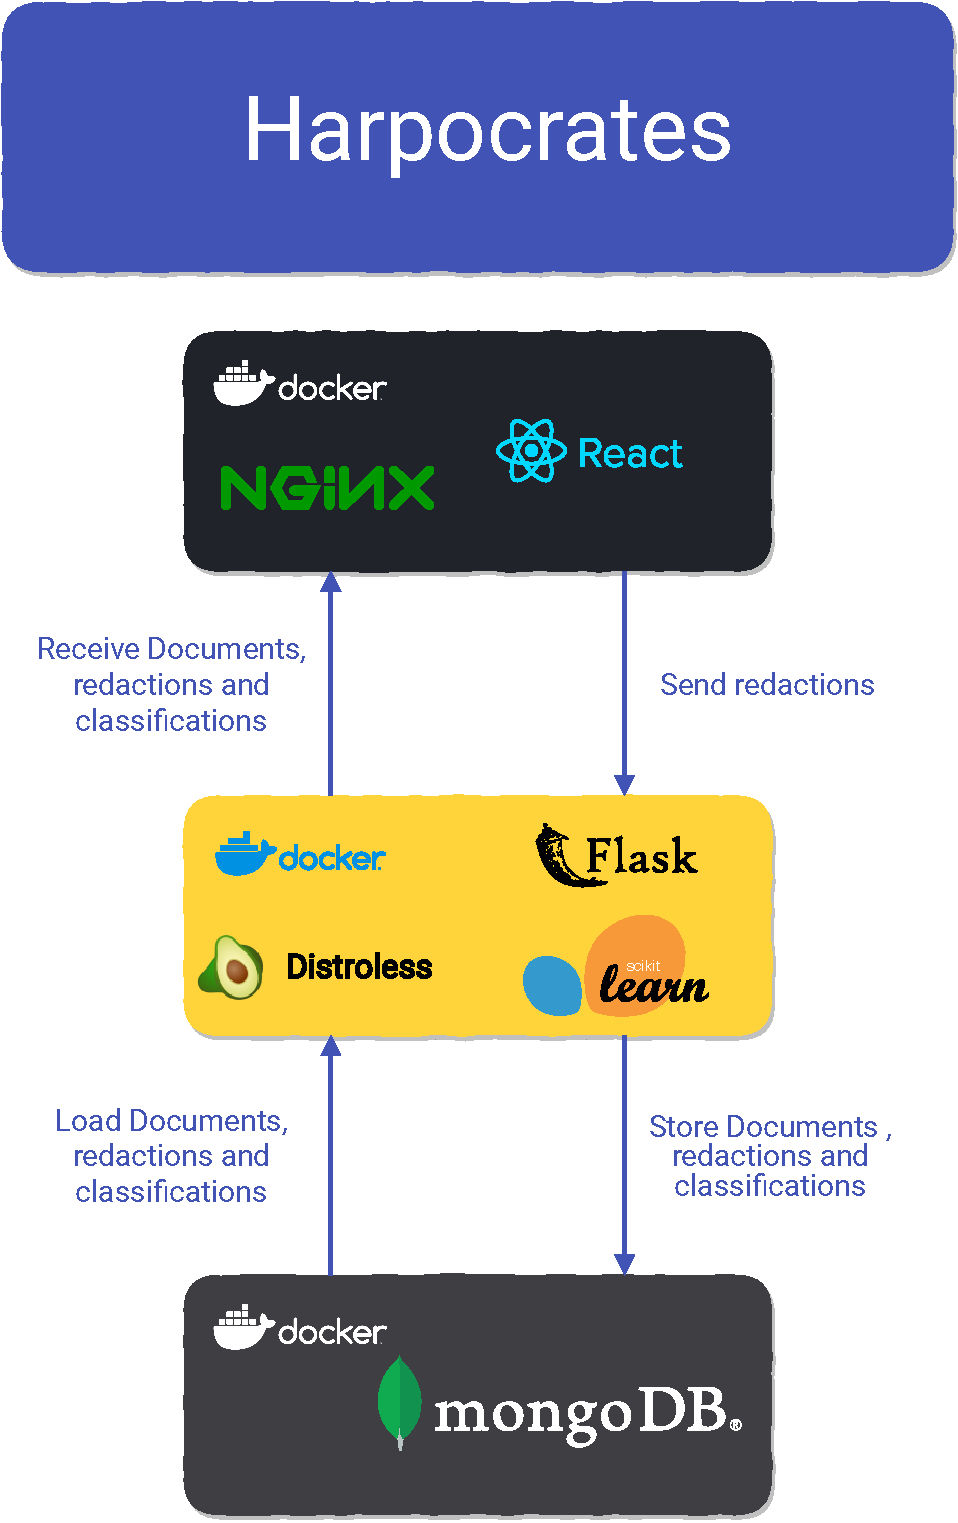
\includegraphics[width=\linewidth]{figures/tech_stack_no_background.pdf}
    \caption{Harpocrates tech stack}\label{fig:tech_stack}
    \vspace{-50pt}
\end{wrapfigure}

% TODO introduce section

Our application's ``stack'' is illustrated in Figure \ref{fig:tech_stack}: it contains three containers.
The first is an \textcite{NGINX2020} web server containers that contains and serves the compiled source code for our ReactJS frontend.
It interacts with a python container which run the Flask API server, this image is based off \textcite{GoogleContainerToolsDistroless2020}'s smaller and more secure ``distroless'' python 3 image \autocite{mooreDistrolessDockerContainerizing2017}.
Lastly, the API uses the official \textcite{MongoDB2020} container as a NoSQL database for storing documents, redactions and classifications.


% TODO show component code and how it gets data from backend

\section{Machine Learning Pipeline}

Our document classifier consists of a number of steps implemented with multiple python libraries assembled in a scikit-learn \verb|Pipeline| (Listing~\ref{listing:ml_pipeline}).

The first step consist in a TF-IDF transformer to convert the document's text to a numeric vector.
We optimized our vectorizer's parameters by performing a grid search with five fold cross-validation to avoid overfitting, the optimal parameter space depends on the use case.

We then resample our highly unbalanced training data with the \textcite{ScikitlearncontribImbalancedlearn2020} library from \textcite{lemaitreImbalancedlearnPythonToolbox2017}.
It implements common resampling techniques \autocite{lemaitreImbalancedlearnPythonToolbox2017}, we use a combination over under and over sampling depending on the use case.
In this example (Listing~\ref{listing:ml_pipeline}), we make use of Synthetic Minority Oversampling TEchnique (SMOTE) oversampling combined with Tomek Link removal undersampling \autocite{batistaStudyBehaviorSeveral2004}.

We use a Support Vector Classifier (SVC) which has performed best for sensitive document classification in past research \autocite{mcdonaldClassifierDigitalSensitivity2014,mcdonaldStudySVMKernel2017}.
We replace scikit-learn's SVC for a parallelized implementation for multicore CPUs and CUDA enabled GPU in order to improve performance \autocite{wenThunderSVMFastSVM2018}.
We also perform a grid search with five fold cross-validation to tune the parameters of the SVC, once again, the optimal parameter space depends on the application.

\begin{listing}[H]
    \inputminted{python}{code/ml_pipeline.py}
    \caption{Machine Learning classification Pipeline}\label{listing:ml_pipeline}
\end{listing}

\section{Classification Explanations}

\begin{listing}[H]
    \inputminted{python}{code/explanations.py}
    \caption{Machine Learning classification explanations}\label{listing:ml_explanations}
\end{listing}


\section{OpenAPI definitions}

\begin{listing}[H]
    \inputminted{yaml}{code/predictedClassification.yml}
    \caption{Defining a predictedClassification response object in OpenAPI}\label{listing:predictedClassification_yml}
\end{listing}

Listing~\ref{listing:predictedClassification_yml} and Listing~\ref{listing:getPredictedClassification_yml} provide an example of an OpenAPI definition of the model of a response along with an accompanying endpoint definition.

One thing to note is that OpenAPI has variable types which can be defined very precisely, allowing for strict type and value checking of variables at both the server and client levels (Listing~\ref{listing:predictedClassification_yml}, line 11-15).

Another interesting aspect of the specification language is that it allows us to define an \verb|object| and extend it with another other \verb|object|.
This object oriented approach allows us to avoid code repetition but also automatically define classes through the code generator.

\begin{listing}[H]
    \inputminted{yaml}{code/getPredictedClassification.yml}
    \caption{Defining a GET endpoint in OpenAPI}\label{listing:getPredictedClassification_yml}
\end{listing}

\section{ReactJS components}

\begin{wrapfigure}{r}{0.45\textwidth}
    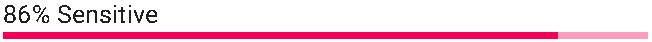
\includegraphics[width=\linewidth]{figures/sensitivity_bar.pdf}
    \caption{Rendered sensitivity bar}\label{fig:sensitivity_bar_preview}
    \vspace{-10pt}
\end{wrapfigure}

ReactJS' latest implementations take a functional approach to web component definition: Listing~\ref{listing:sensitivity_bar} demonstrates this with one of the simpler components of our application (Figure~\ref{fig:sensitivity_bar_preview}).

One of the features of ReactJS is its ``one-way data binding'' that is data is passed from parent to child component using a \verb|props| dictionary.
In Listing~\ref{listing:sensitivity_bar}, we pass a document's classification to the \verb|SensitivityBar| component to change its appearance based on its sensitivity value.
This one way data binding simplifies the flow of information thus making them easier to debug.


\begin{listing}[H]
    \inputminted{jsx}{code/documentSensitivityBar.js}
    \caption{Document sensitivity bar}\label{listing:sensitivity_bar}
\end{listing}

\section{Version-Control and Continuous Integration}

Throughout the project, we tried various repository organizations, hosted git platforms and Continuous Integration (CI) tools.


\subsection{Mono-repository}

Initially, we setup our project as multiple repositories within a group on \href{https://gitlab.com/harpocrates-app}{gitlab.com}, thus holding the frontend, server, api client and specification in their own repositories.
However, the repository management overhead introduced was too complex. A change in the specification would imply a commit in all 3 other repositories.
To counter this, we shifted to a project ``monorepository'' which provide ``better managing of cross-project changes, easy refactoring, simplified organization'' \autocite[1]{britoMonoreposMultivocalLiterature2018}.

\subsection{Continuous Integration}

We chose \href{https://gitlab.com/}{gitlab.com} because of its powerful and well documented Continuous Integration (CI) capabilities.
We made use of these features in order to automatically build and test the the OpenAPI specification, docker containers and the documentation for each commit we setup a CI Pipeline (Figure~\ref{fig:ci}) .

\begin{figure}[H]
    %TODO use PDF/PNG this look ugly
    \centering
    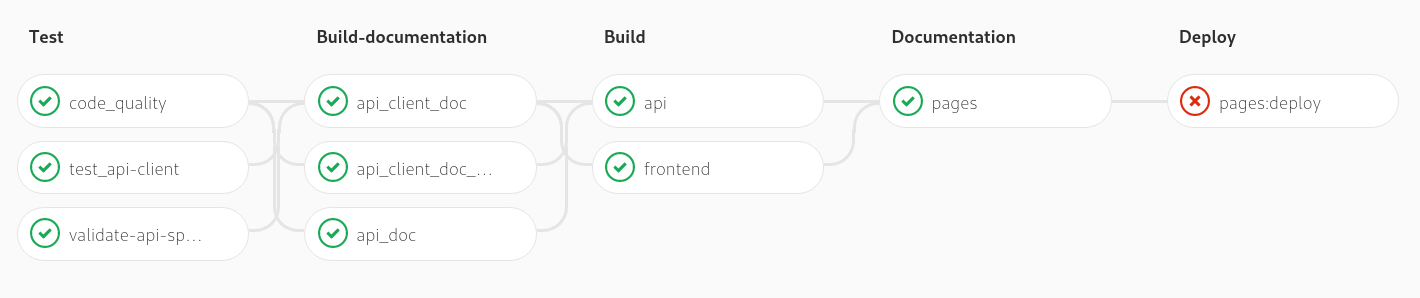
\includegraphics[width=0.9\linewidth]{figures/ci.png}
    \caption{CI Pipeline}\label{fig:ci}
\end{figure}

In a first \verb|test| stage we test our API specification, the accompanying API client and run a code quality check using \textcite{Codeclimate2020} to check for common programming mistakes.

In the \verb|build-documentation| stage build the documentation for our API, its client and the general application as static web pages that are later auto published at \href{https://harpocrates-app.gitlab.io/harpocrates/}{harpocrates-app.gitlab.io/harpocrates} with Gitlab Pages in the \verb|deploy| stage.

Most importantly, the \verb|build| stage builds the docker containers for our frontend and API.
Once the images are built, they are tagged with either the branch name, or the commit hash and published on a \href{https://gitlab.com/harpocrates-app/harpocrates/container_registry}{docker container registry hosted on gitlab.com}.

\subsection{Github bots and integrations}

We later moved our main repository to \href{https://github.com/guillaumedsde/Harpocrates}{github.com}, to make use of multiple helper bots on Github while keeping a mirror of the repository on Gitlab to avoid redifining our CI Pipeline.

During development, multiple of our libraries received updates.
To avoid having to hunt down and keep track of updates, we set up \textcite{Dependabot2020}, to automatically create Pull Requests (PR) on our repository for dependency updates.

We also kept track of our tests' code coverage for each Pull Request using \textcite{Codecov2020}.
It is another Github bot that calculates code coverage for every commit and posts code coverage changes in PRs.

%==================================================================================================================================
\chapter{Evaluation}

% link back to requirements,  how have they been met?
% Expert panel testing
% unit testing

\section{Code Testing}

\section{Expert Panel}

\section{User Study}

We conducted a user evaluation in order to evaluate the effectiveness of our application in helping reviewers conduct a sensitivity review. We sought to answer a handful of research questions:

\begin{enumerate}[label=\textbf{RQ\arabic*}]
    \item Does our visualization of predicted document sensitivity and explanation features help reviewers conduct a sensitivity review faster?
    \item Does it improve the accuracy of the sensitivity review process?
    \item Does it improve reviewers' confidence in the completeness of their sensitivity review?
\end{enumerate}

\subsection{Preparations and Experimental Setup}

\section{Dataset and classifier experimentations}

Our collection is a set of 3801 Government documents relating to International Activities sensitivity assessed by government sensitivity reviewers.
The ground truth for document sensitivity was established with respect to sections 40 (S40, Personal Information) and 27 (S27, International Relations) of the Freedom of Information Act (FOIA).
This appraisal resulted in 502 (13\%) documents deemed sensitive to either S40, S27 or both with 3299 non sensitive documents (87\%).

Due to our lack of access to expert document reviewers, we conducted our study with students either from an academic Politics background or with International Relations awareness.
We focus on identifying ``Personal Information'' exceptions to the FOIA which we deem more ``attainable'' given our non-expert test subjects.

Our dataset contains 289 documents with S40 exemptions, we split the collection in order to obtain a stratified sample ``test set'' 20\% the size of the entire collection.
We vectorize the remaining 80\% ``train set'' using Scikit-Learn's \verb|TfidfVectorizer|.
We resamplethe resulting vectors to achieve better class balance with imblearn's \verb|SMOTEENN|, a combination of majority class downsampling and minority class upsampling \autocite{lemaitreImbalancedlearnPythonToolbox2017}.
We use the resulting collection of resampled vectors to train a SVC for binary classification of documents depending on whether or not they contain sensitive information.
Table \ref{tab:clf_perf} shows the results we obtained while trying to find a classifier with satisfactory performance for our user study.

\begin{table}[H]
    \begin{adjustbox}{width=\textwidth,center}
        \begin{tabular}{l|llllll}
            Classification pipeline                  & Tuned For & FOIA   & BAC    & F2     & Precision & Recall \\ \hline
            CountVectorizer, RandomUnderSampler, SVC &           & 27, 40 & 0.4993 & 0.0847 & 0.0262    & 0.1920 \\
            CountVectorizer, SMOTE, SVC              &           & 27, 40 & 0.4856 & 0.1549 & 0.1151    & 0.1829 \\
            TF-IDF, SMOTEENN, SVC                    & BAC       & 40     & 0.5576 & 0.1182 & 0.0659    & 0.1911 \\
            TF-IDF, SMOTEENN, SVC                    & F2        & 40     & 0.5482 & 0.1331 & 0.0385    & 0.4047 \\
            TF-IDF, RandomUnderSampler, SVC          & BAC       & 27, 40 & 0.5526 & 0.3593 & 0.1669    & 0.5454 \\
            TF-IDF, RandomUnderSampler, SVC          & F2        & 27, 40 & 0.5079 & 0.4359 & 0.1340    & 0.9980 \\
        \end{tabular}
    \end{adjustbox}
    \caption{Best performing classifiers using 5-fold cross validation targeting different metrics and sensitive classifications}\label{tab:clf_perf}
\end{table}

Due to time constraints, we only sample documents to review from the test set that are under 2000 characters.
We then selected both sensitive and non-sensitive documents in order to represent every category of the confusion matrix for the classifier with the following counts:

\begin{table}[H]
    \centering
    \begin{tabular}{l|ll}
                                & Actually non-sensitive & Actually Sensitive \\ \hline
        Predicted non-sensitive & 3                      & 1                  \\
        Predicted Sensitive     & 1                      & 1
    \end{tabular}
    \caption{Count of selected documents in the classifier's confusion matrix}\label{tab:confusion-matrix-selection}
\end{table}

We sample test documents accordingly twice: once for each User Interface (UI).
One interface \textit{test mode 1} (Figure~\ref{fig:test-mode-1}) is a simplified version of the final interface containing the classification prediction and the accompanying explanations.
The other, \textit{test mode 2} (Figure~\ref{fig:test-mode-2}) is a stripped down version that only displays the document, and the manual redaction tools (document title and sensitivity type selection).

\begin{figure}[H]
    \centering
    \begin{subfigure}[c]{0.49\textwidth}
        \centering
        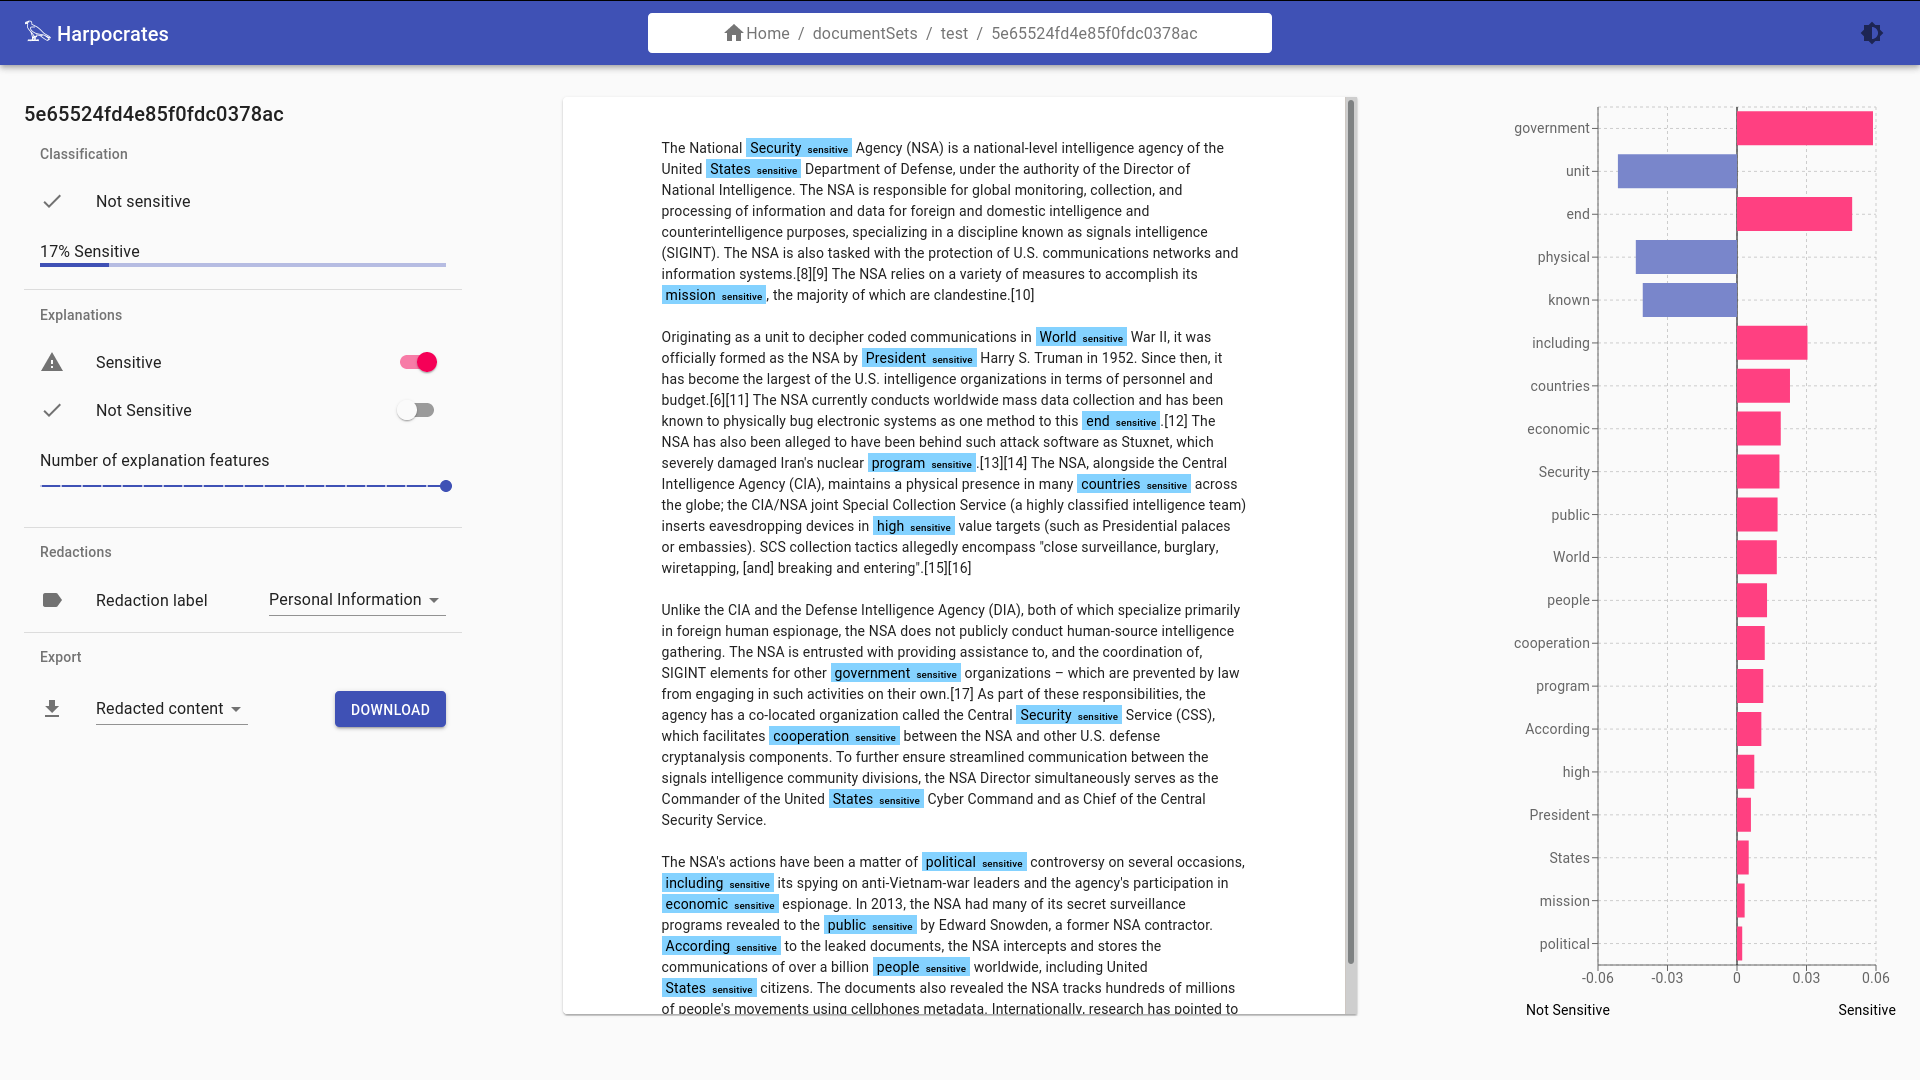
\includegraphics[width=\textwidth]{images/ui_test_mode_1.png}
        \caption{Test mode 1}\label{fig:test-mode-1}
    \end{subfigure}
    \begin{subfigure}[c]{0.49\textwidth}
        \centering
        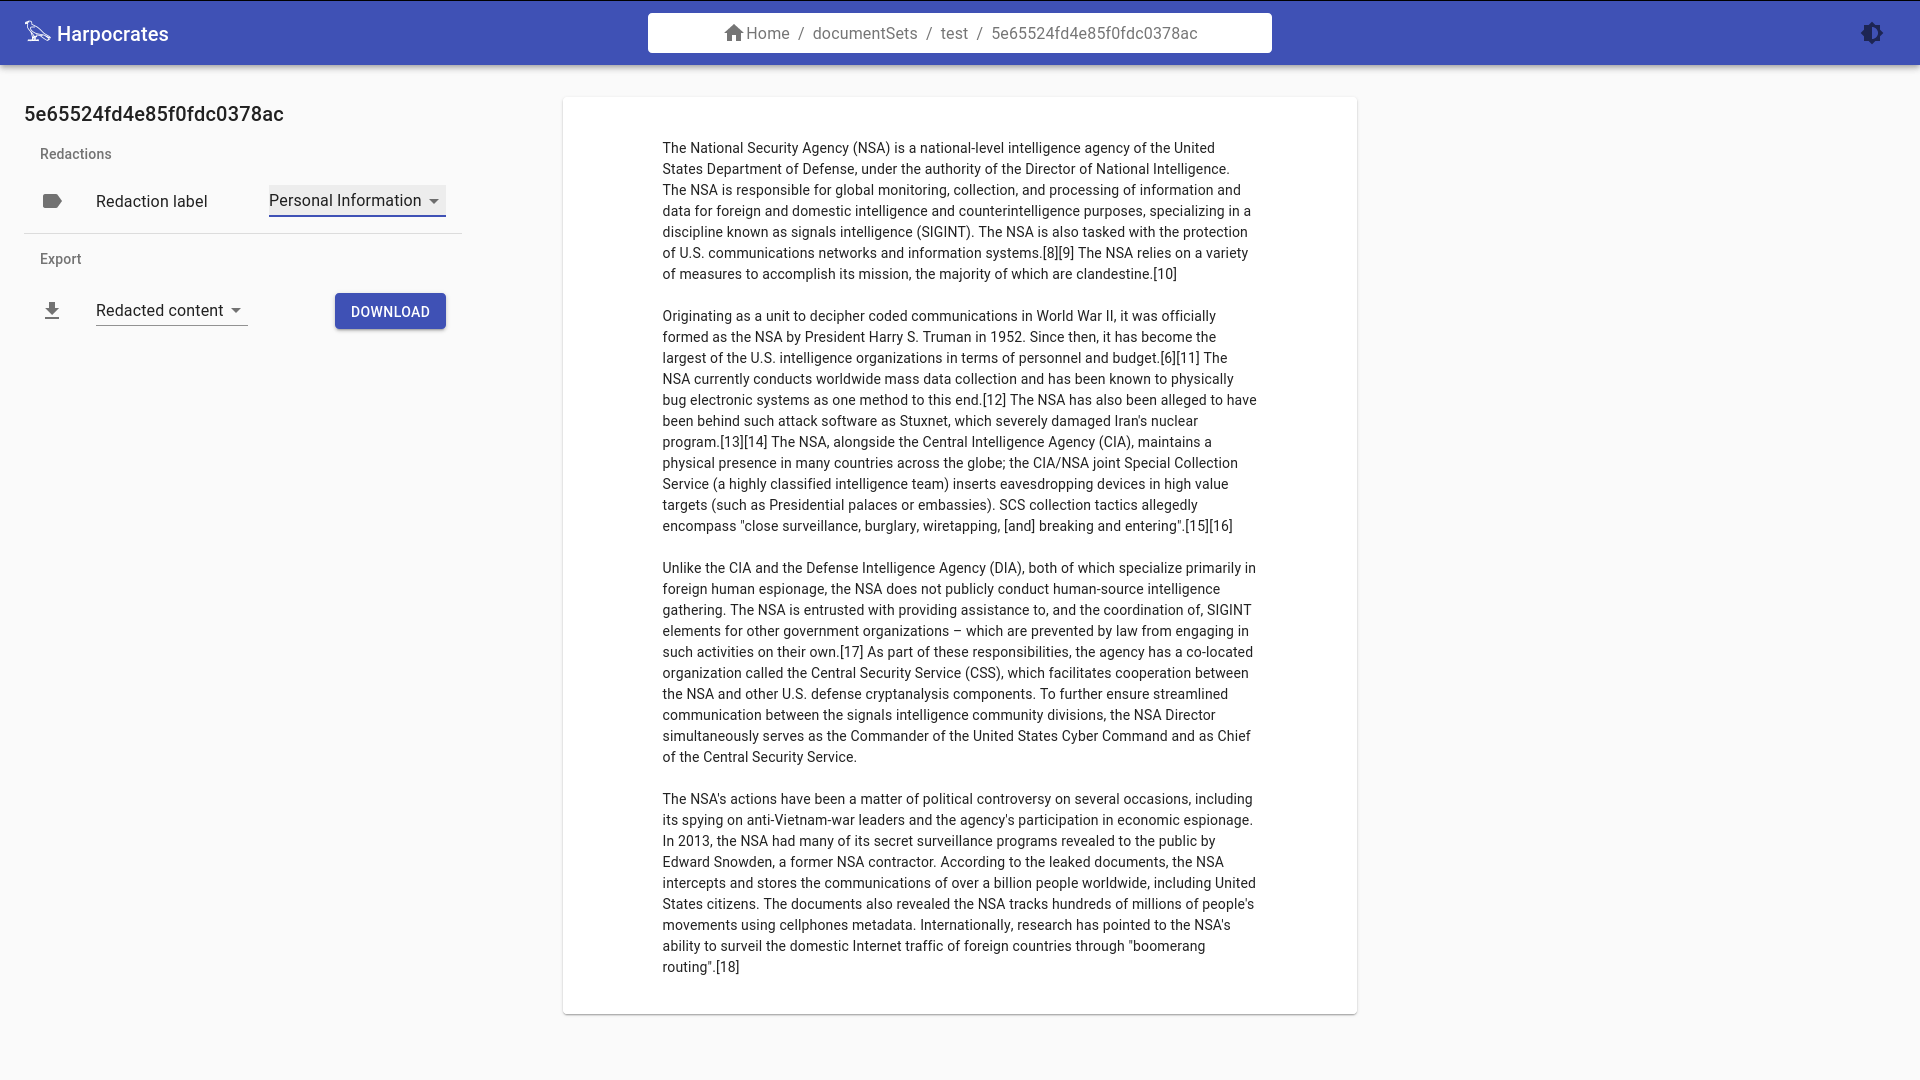
\includegraphics[width=\textwidth]{images/ui_test_mode_2.png}
        \caption{Test mode 2}\label{fig:test-mode-2}
    \end{subfigure}
    \caption{The two test modes used for evaluation}\label{fig:test-modes}
\end{figure}

We asked our participants to review each set of test documents with one of the two interfaces.
The starting interface and the document order within each set was chosen randomly in to minimize the learning effect on the reviewing task.
After each batch of documents, we handed our reviewers sections of a questionnaire (Appendix~\ref{appendix:questionnaire}) to record their impressions about the interface, confidence about their work and time to review each document.
This questionnaire is split into three sections, the first two were an identical based on the System Usability Survey (SUS) format \autocite[Chap.~21]{jordanUsabilityEvaluationIndustry1996} which aimed at evaluating the interface as a whole.
The first two sections were answered after each review batch was completed, then, the last section was handed out.
It seeks to evaluate the usefulness of each invidual component in interface 1.

\subsection{Results}

As mentioned, each user is asked to review one collection of six documents for personal information sensitivities (FOIA Section 40) for each user interface.
The independent variables will a set of two user interfaces: with and without the predicted classification and explanations (more details below) which all users will both use. We will measure multiple dependent variables against our two interfaces (the independant variables):

\begin{itemize}
    \item Firstly, we measure the time to review each document in both collections.
          We normalize document review time with the document's word count in order to account for differing document length, although it should be noted that a simple word count does not necessarily reflect the complexity of a document, especially for sensitivity review.
    \item Secondly we record the accuracy of each reviewer on each interface for all documents.
          We extract two measures from our participants' review batches: the balanced accuracy and \(F_{2}\), measures particularly well suited to evaluating sensitivity review \autocite{mcdonaldStudySVMKernel2017}.
    \item Lastly, we evaluate the confidence of the reviewers after using each interface with a Likert scale in the questionnaires.
\end{itemize}

% t-test for review time (because time is a continuous variable)
Regarding \textbf{RQ1}, we hypothesise that \textit{There is a statistically significant improvement to the document review time with interface 1} (\textbf{H1}) along with a null hypothesis stating that \textit{There is no statistically significant improvement to the document review time with interface 1} (\(\mathbf{H1_{null}}\)) .
To evaluate this, we perform a paired sample one-tailed Student's T-Test, pairing review times of a given document on interface 1 and on interface 2.
Since we randomely alternate between both interfaces we are able to pair all review times for a document reviewed on interface 1 with another review time for that same document on interface 2.
Ideally, we expect our p-value to be lower than our critical value at a 95\% confidence level, allowing us to confirm \textbf{H1} for our sample.

In answer to \textbf{RQ2} we suggest that \textit{Interface 1 significantly improves the the accuracy of reviewers} (\textbf{H2}) with our null hypothesis thus being that \textit{Interface 1 does not significantly improve the the accuracy of reviewers} (\(\mathbf{H2_{null}}\)).
To confirm \textbf{H2} or \(\mathbf{H2_{null}}\), we evaluate the significance for both the difference in balanced accuracy and \(F_{2}\) measure at 95\% confidence.
Since Interface 1 essentially contains a predicted sensitivity which might be taken as a guideline by our participants, we assume an unequal variance in distribution of review performance in interface 1 and 2.
Indeed, we expect the accuracy for documents reviewed with interface 1 to be more ``clustered'' together: namely around the classifier's predicted sensitivity.
Once again, we perform a paired sample one-tailed Student's T-Test, pairing performance for a given document on interface 1 with that same metric and document on interface 2.

Lastly, we suppose that \textit{Interface 1 significantly improves the the confidence of participants in the quality of their sensitivity review} (\textbf{H3}) or that \textit{Interface 1 does no significantly improves the the confidence of participants in the quality of their sensitivity review} (\(\mathbf{H3_{null}}\)) in response to \textbf{RQ3}.
Since our sample size is expectedly quite restricted, we prefer Fisher's exact test over a Chi-square test for testing the significance of the difference in confidence between interface 1 and 2 to validate \textbf{H3} or \(\mathbf{H3_{null}}\).
%TODO finish detailing fisher's exact test

%==================================================================================================================================
\chapter{Conclusion}


% requirements I've met
% reflections
% future work

%==================================================================================================================================
%
% 
%==================================================================================================================================
%  APPENDICES  

\begin{appendices}
    % \settocdepth{chapter}
    \chapter{PDF Editors}
    \section{PhantomPDF context menu}\label{fig:foxit-menu}
    \begin{figure}[H]
        \centering
        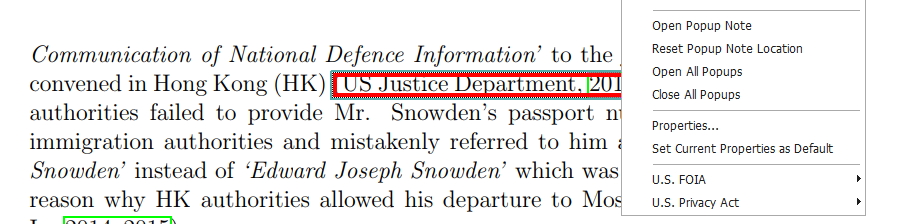
\includegraphics[width=0.7\linewidth]{images/related_products/foxit_redaction.png}
    \end{figure}
    \section{PhantomPDF redact all}\label{fig:foxit-redact-all}
    \begin{figure}[H]
        \centering
        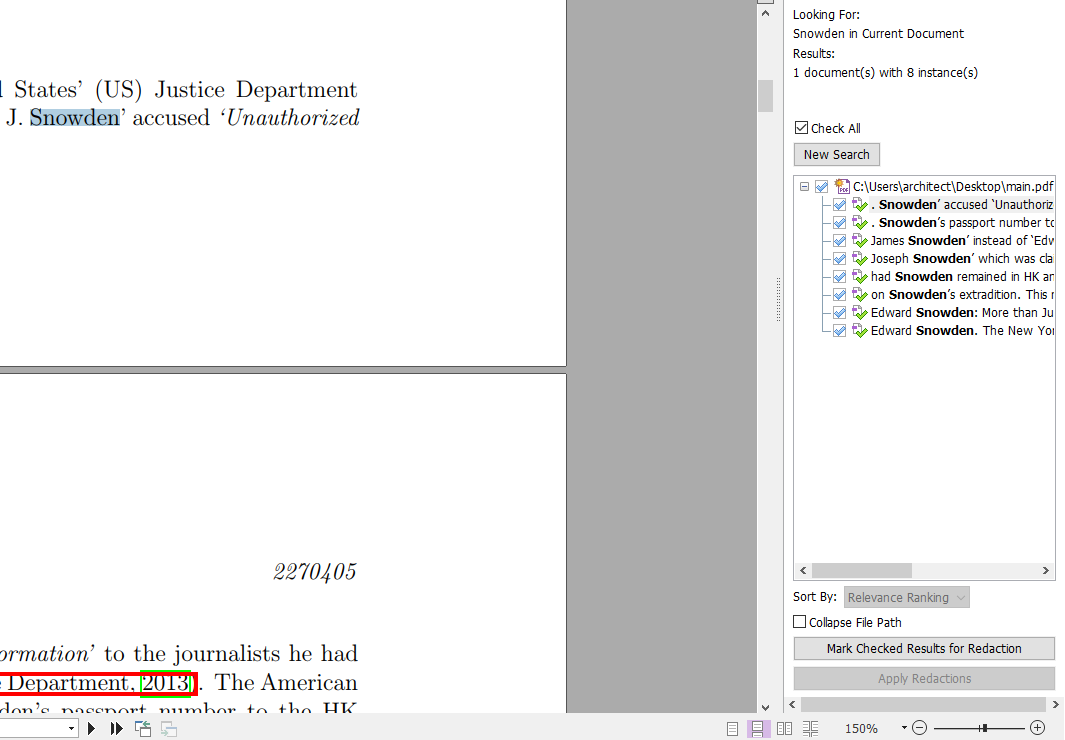
\includegraphics[width=0.7\linewidth]{images/related_products/foxit_redact_all.png}
    \end{figure}
    \section{Adobe Acrobat redact all}\label{fig:adobe-redact-all}
    \begin{figure}[H]
        \centering
        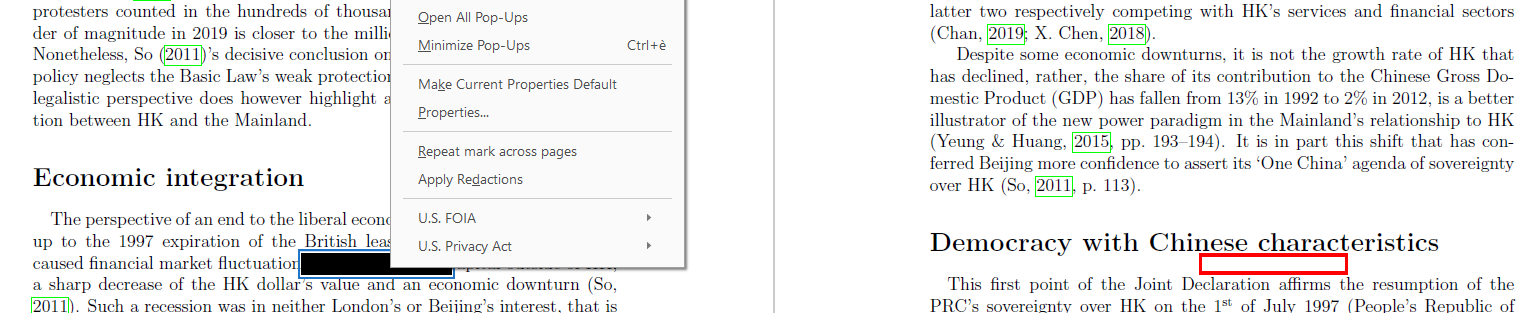
\includegraphics[width=\linewidth]{images/related_products/adobe_redact_all.png}
    \end{figure}
    \chapter{Wireframes}
    \section{Homepage}
    \begin{figure}[H]
        \centering
        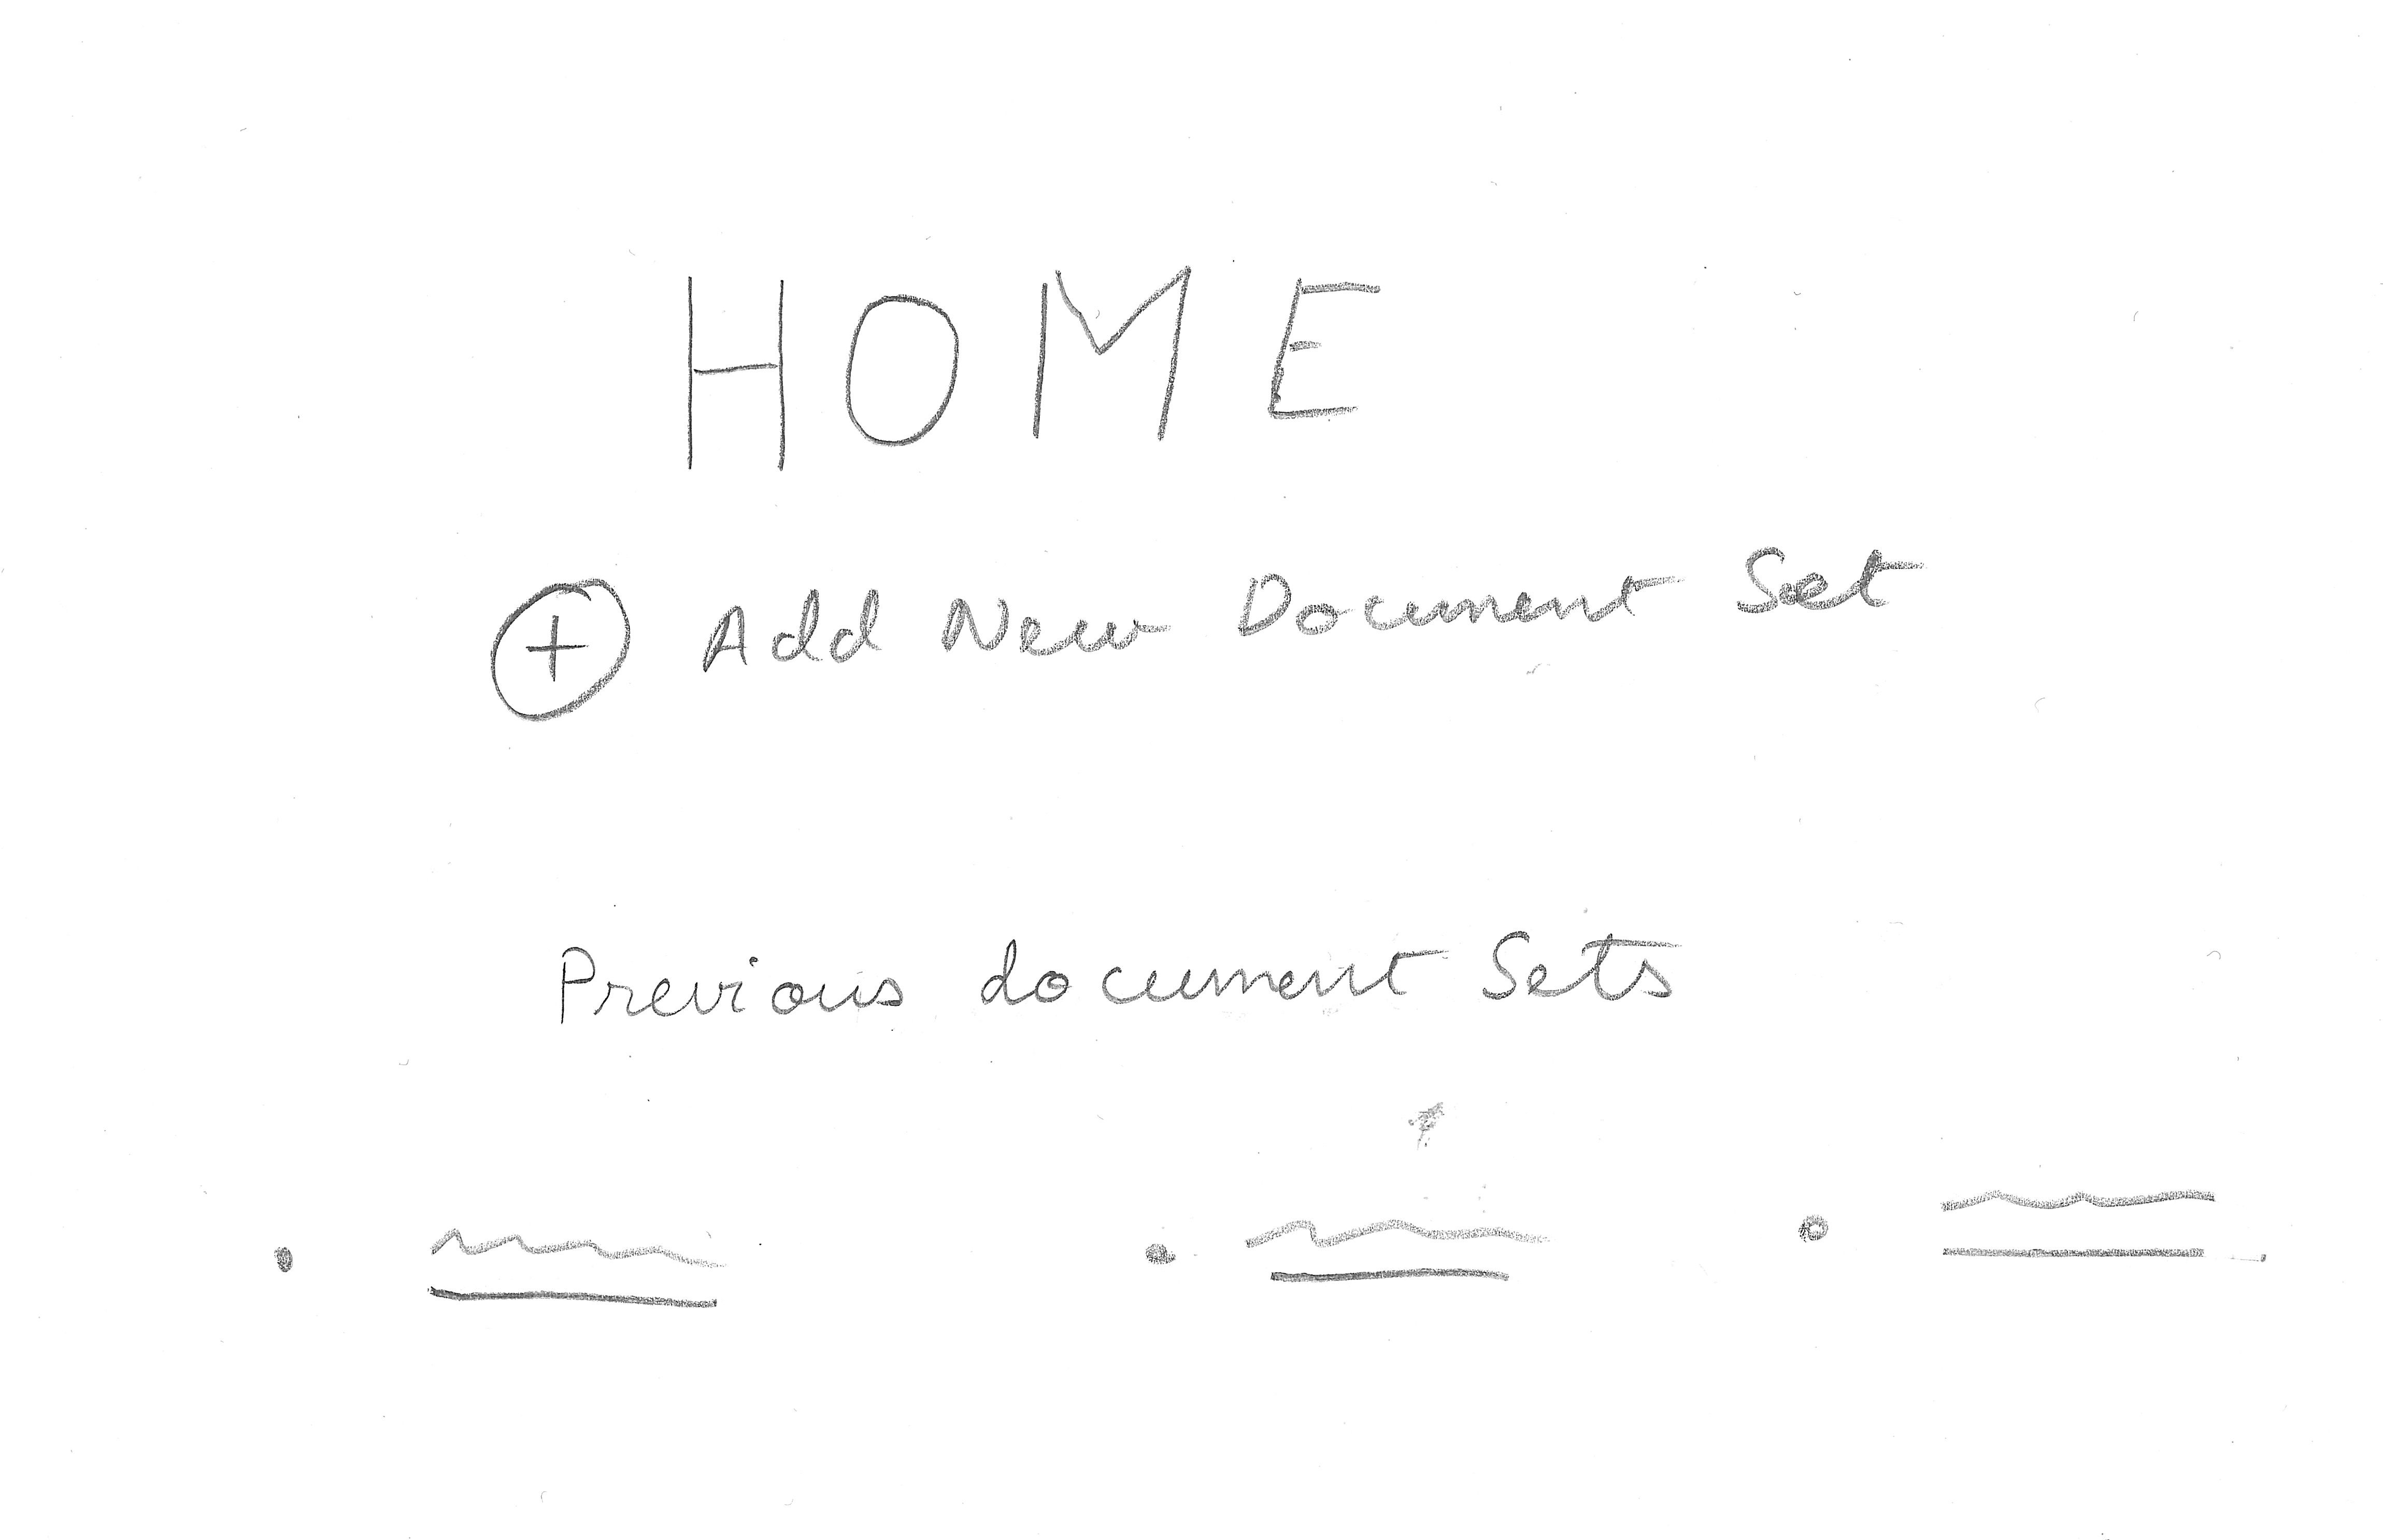
\includegraphics[width=0.7\linewidth]{images/wireframes/home.jpg}
    \end{figure}
    \section{Set View}
    \begin{figure}[H]
        \centering
        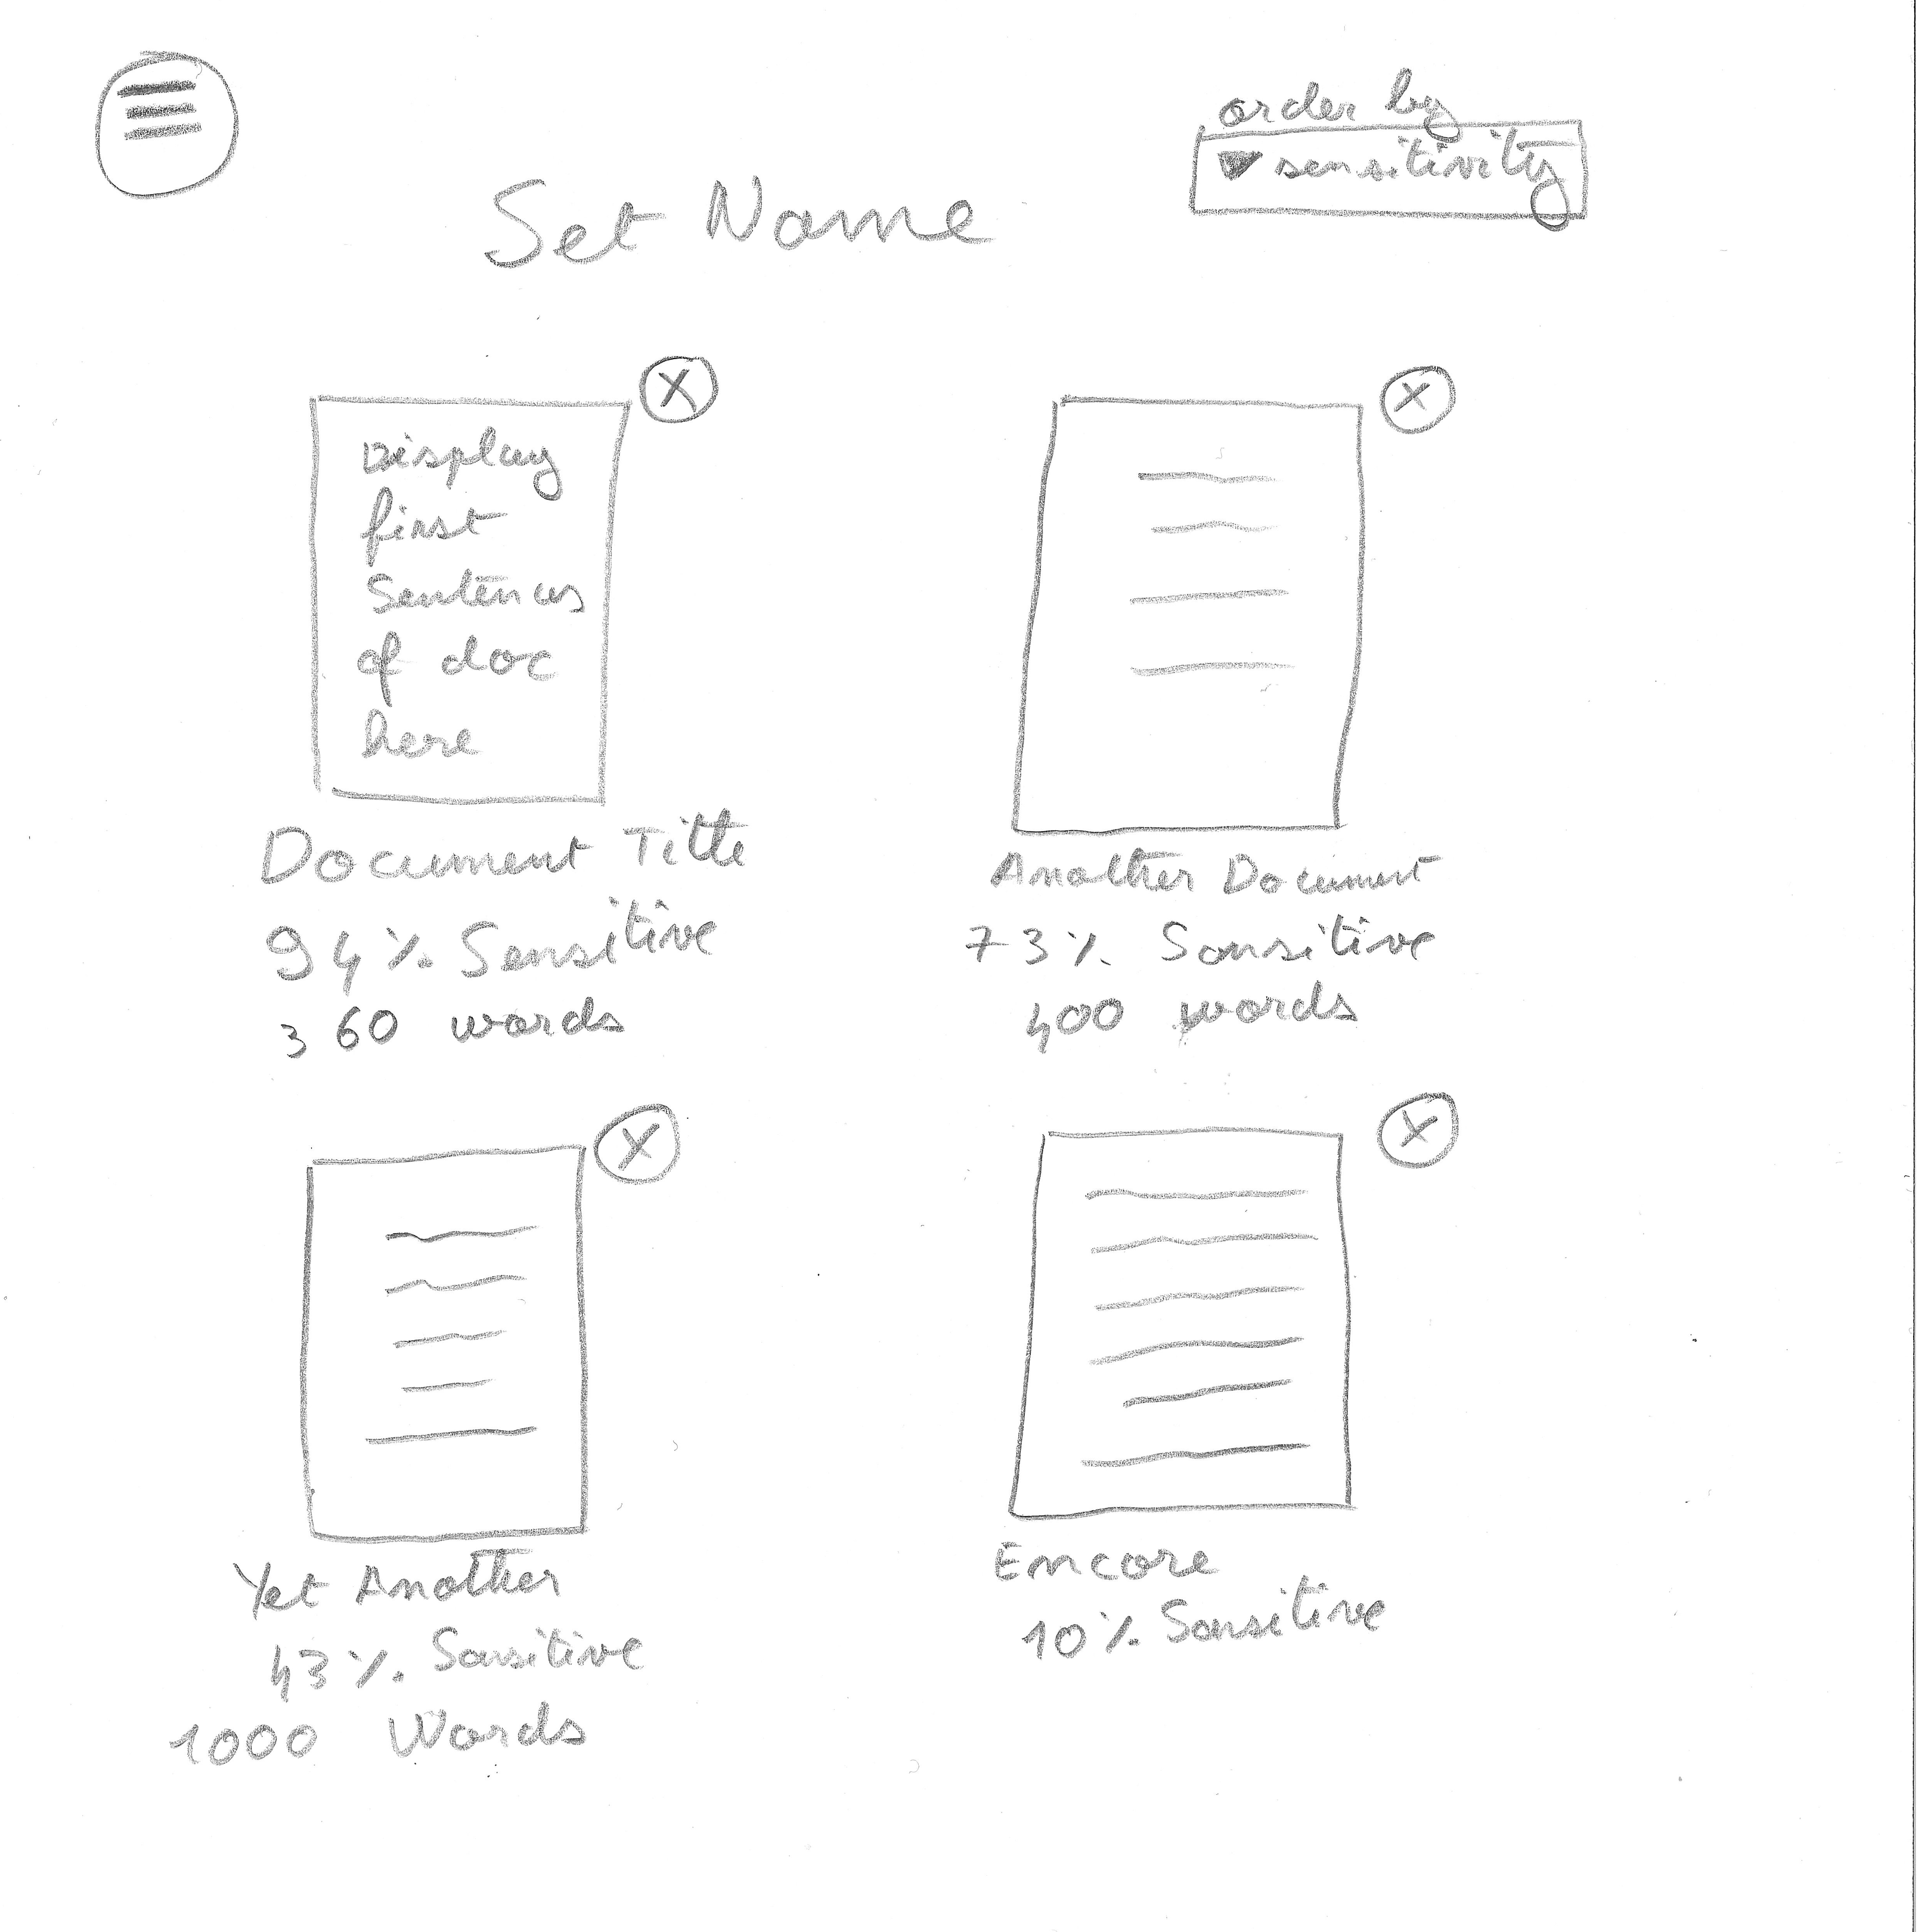
\includegraphics[width=0.65\linewidth]{images/wireframes/set.jpg}
    \end{figure}
    \section{Set View - opened menu}
    \begin{figure}[H]
        \centering
        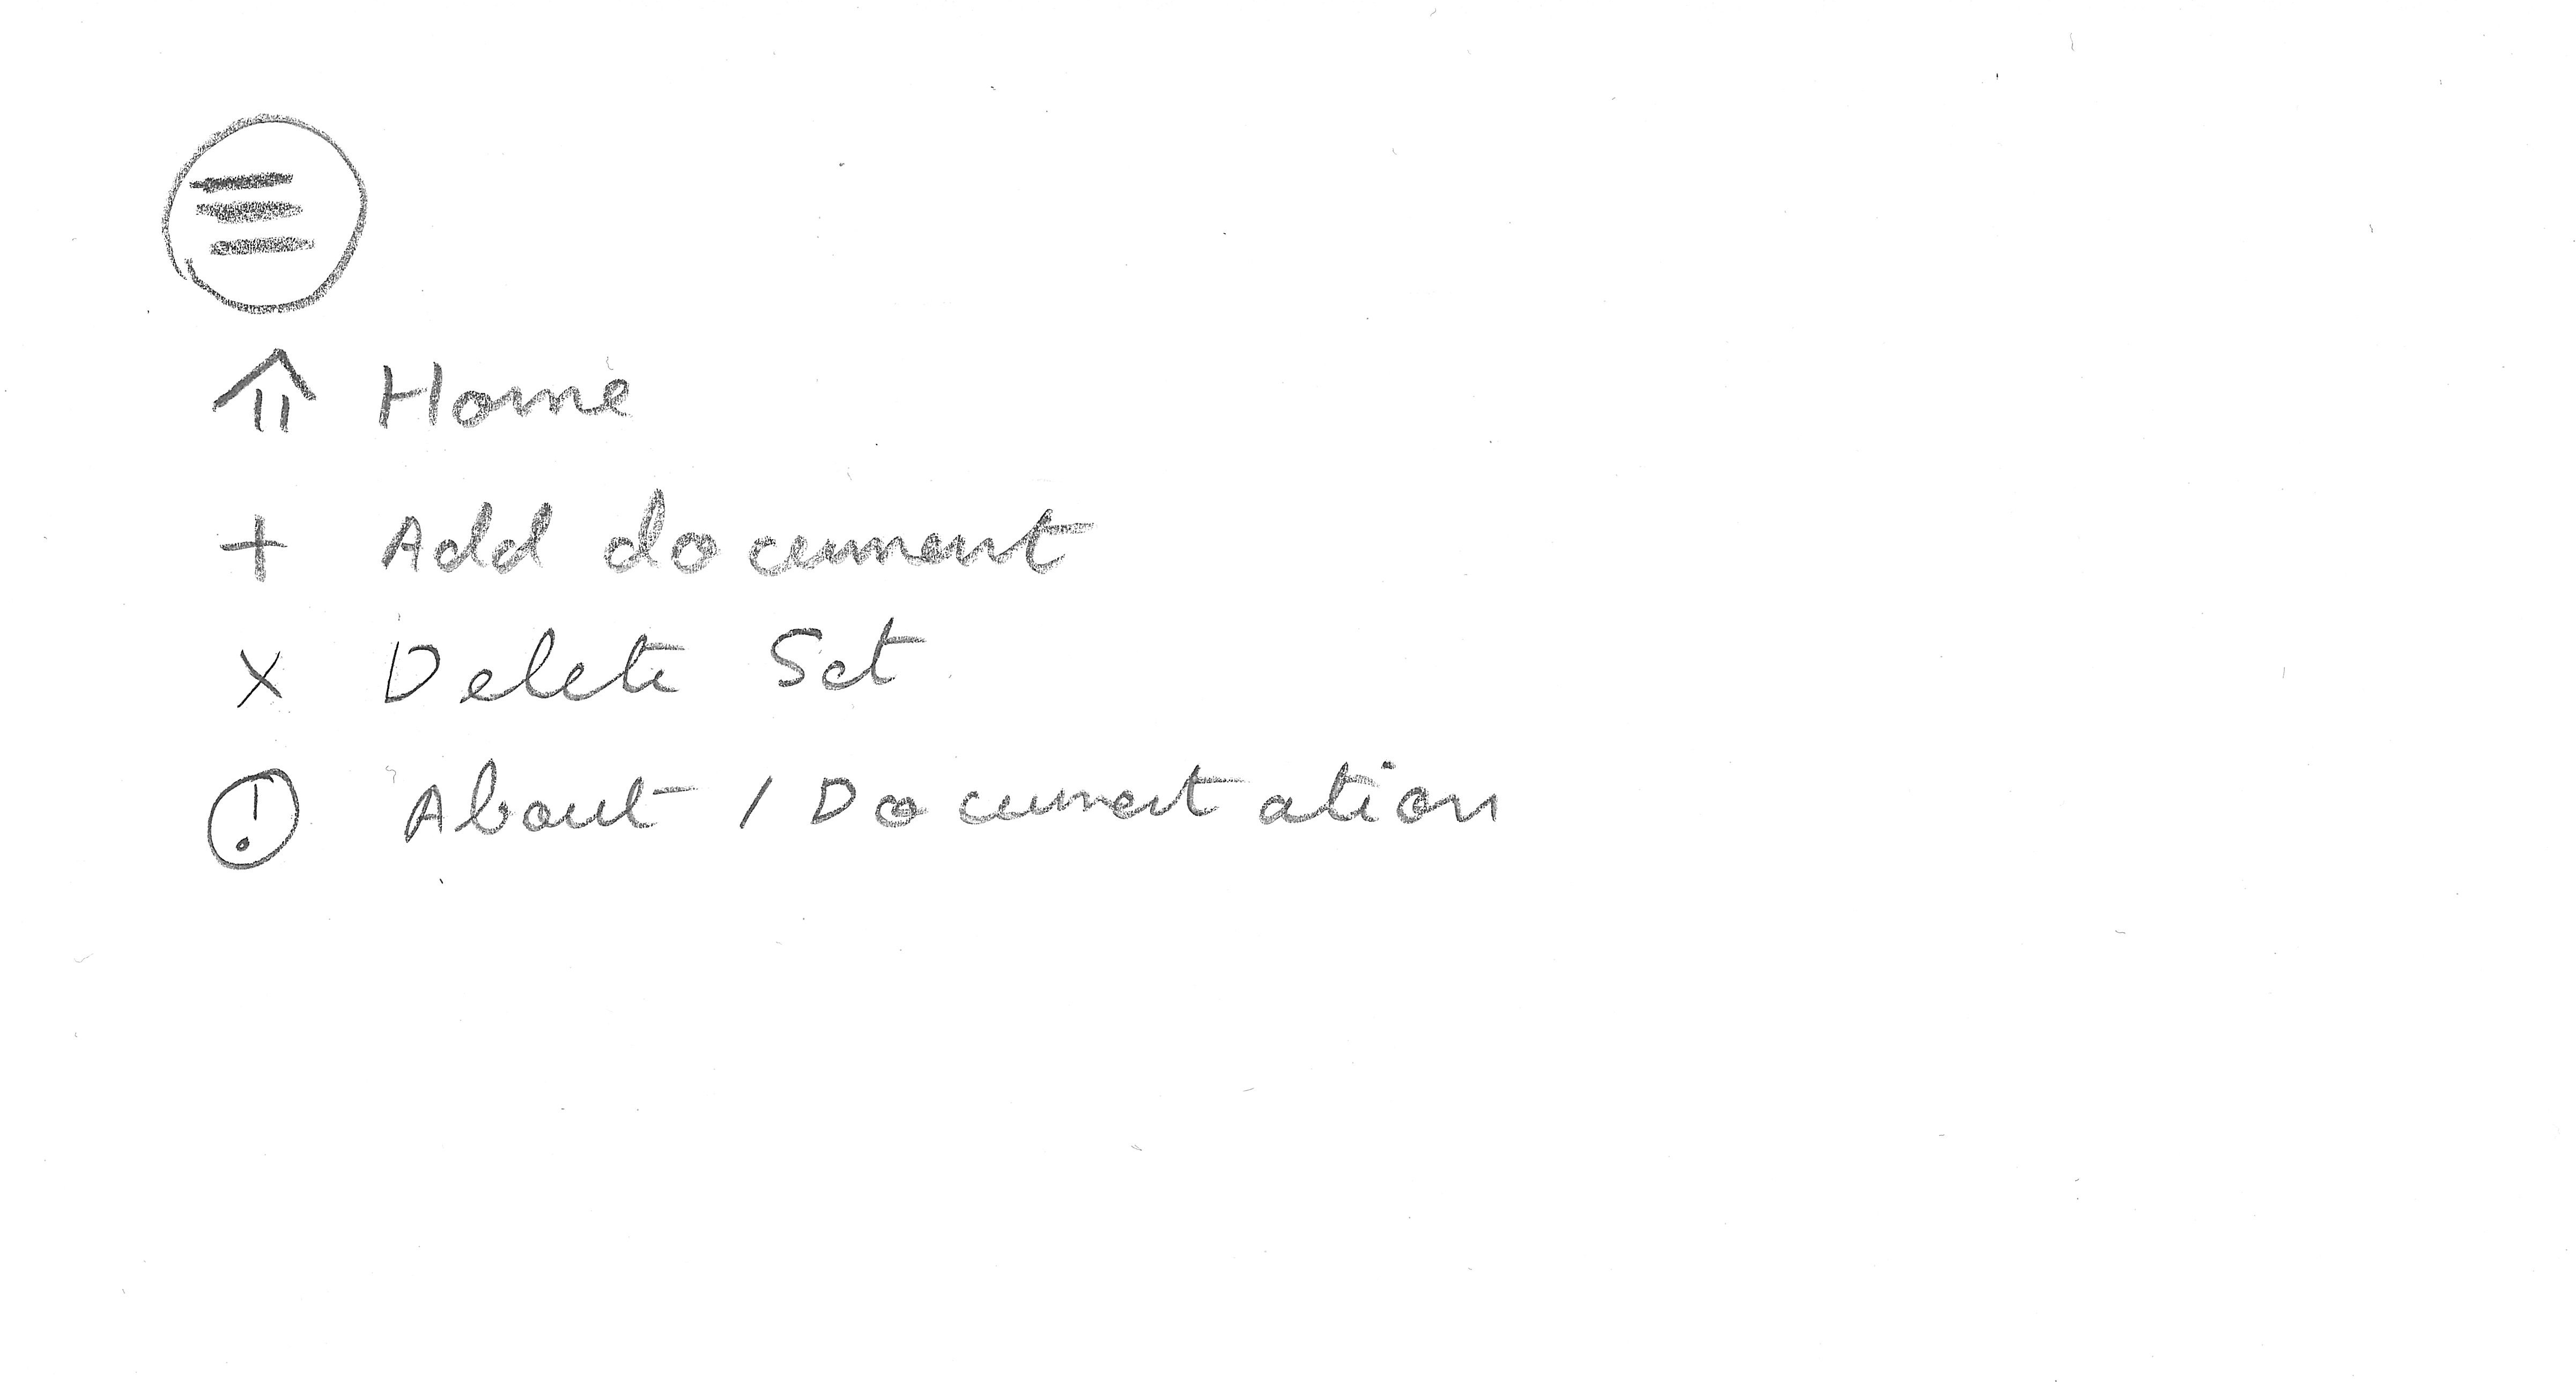
\includegraphics[width=\linewidth]{images/wireframes/set-menu.jpg}
    \end{figure}
    \section{Document View v1}
    \begin{figure}[H]
        \centering
        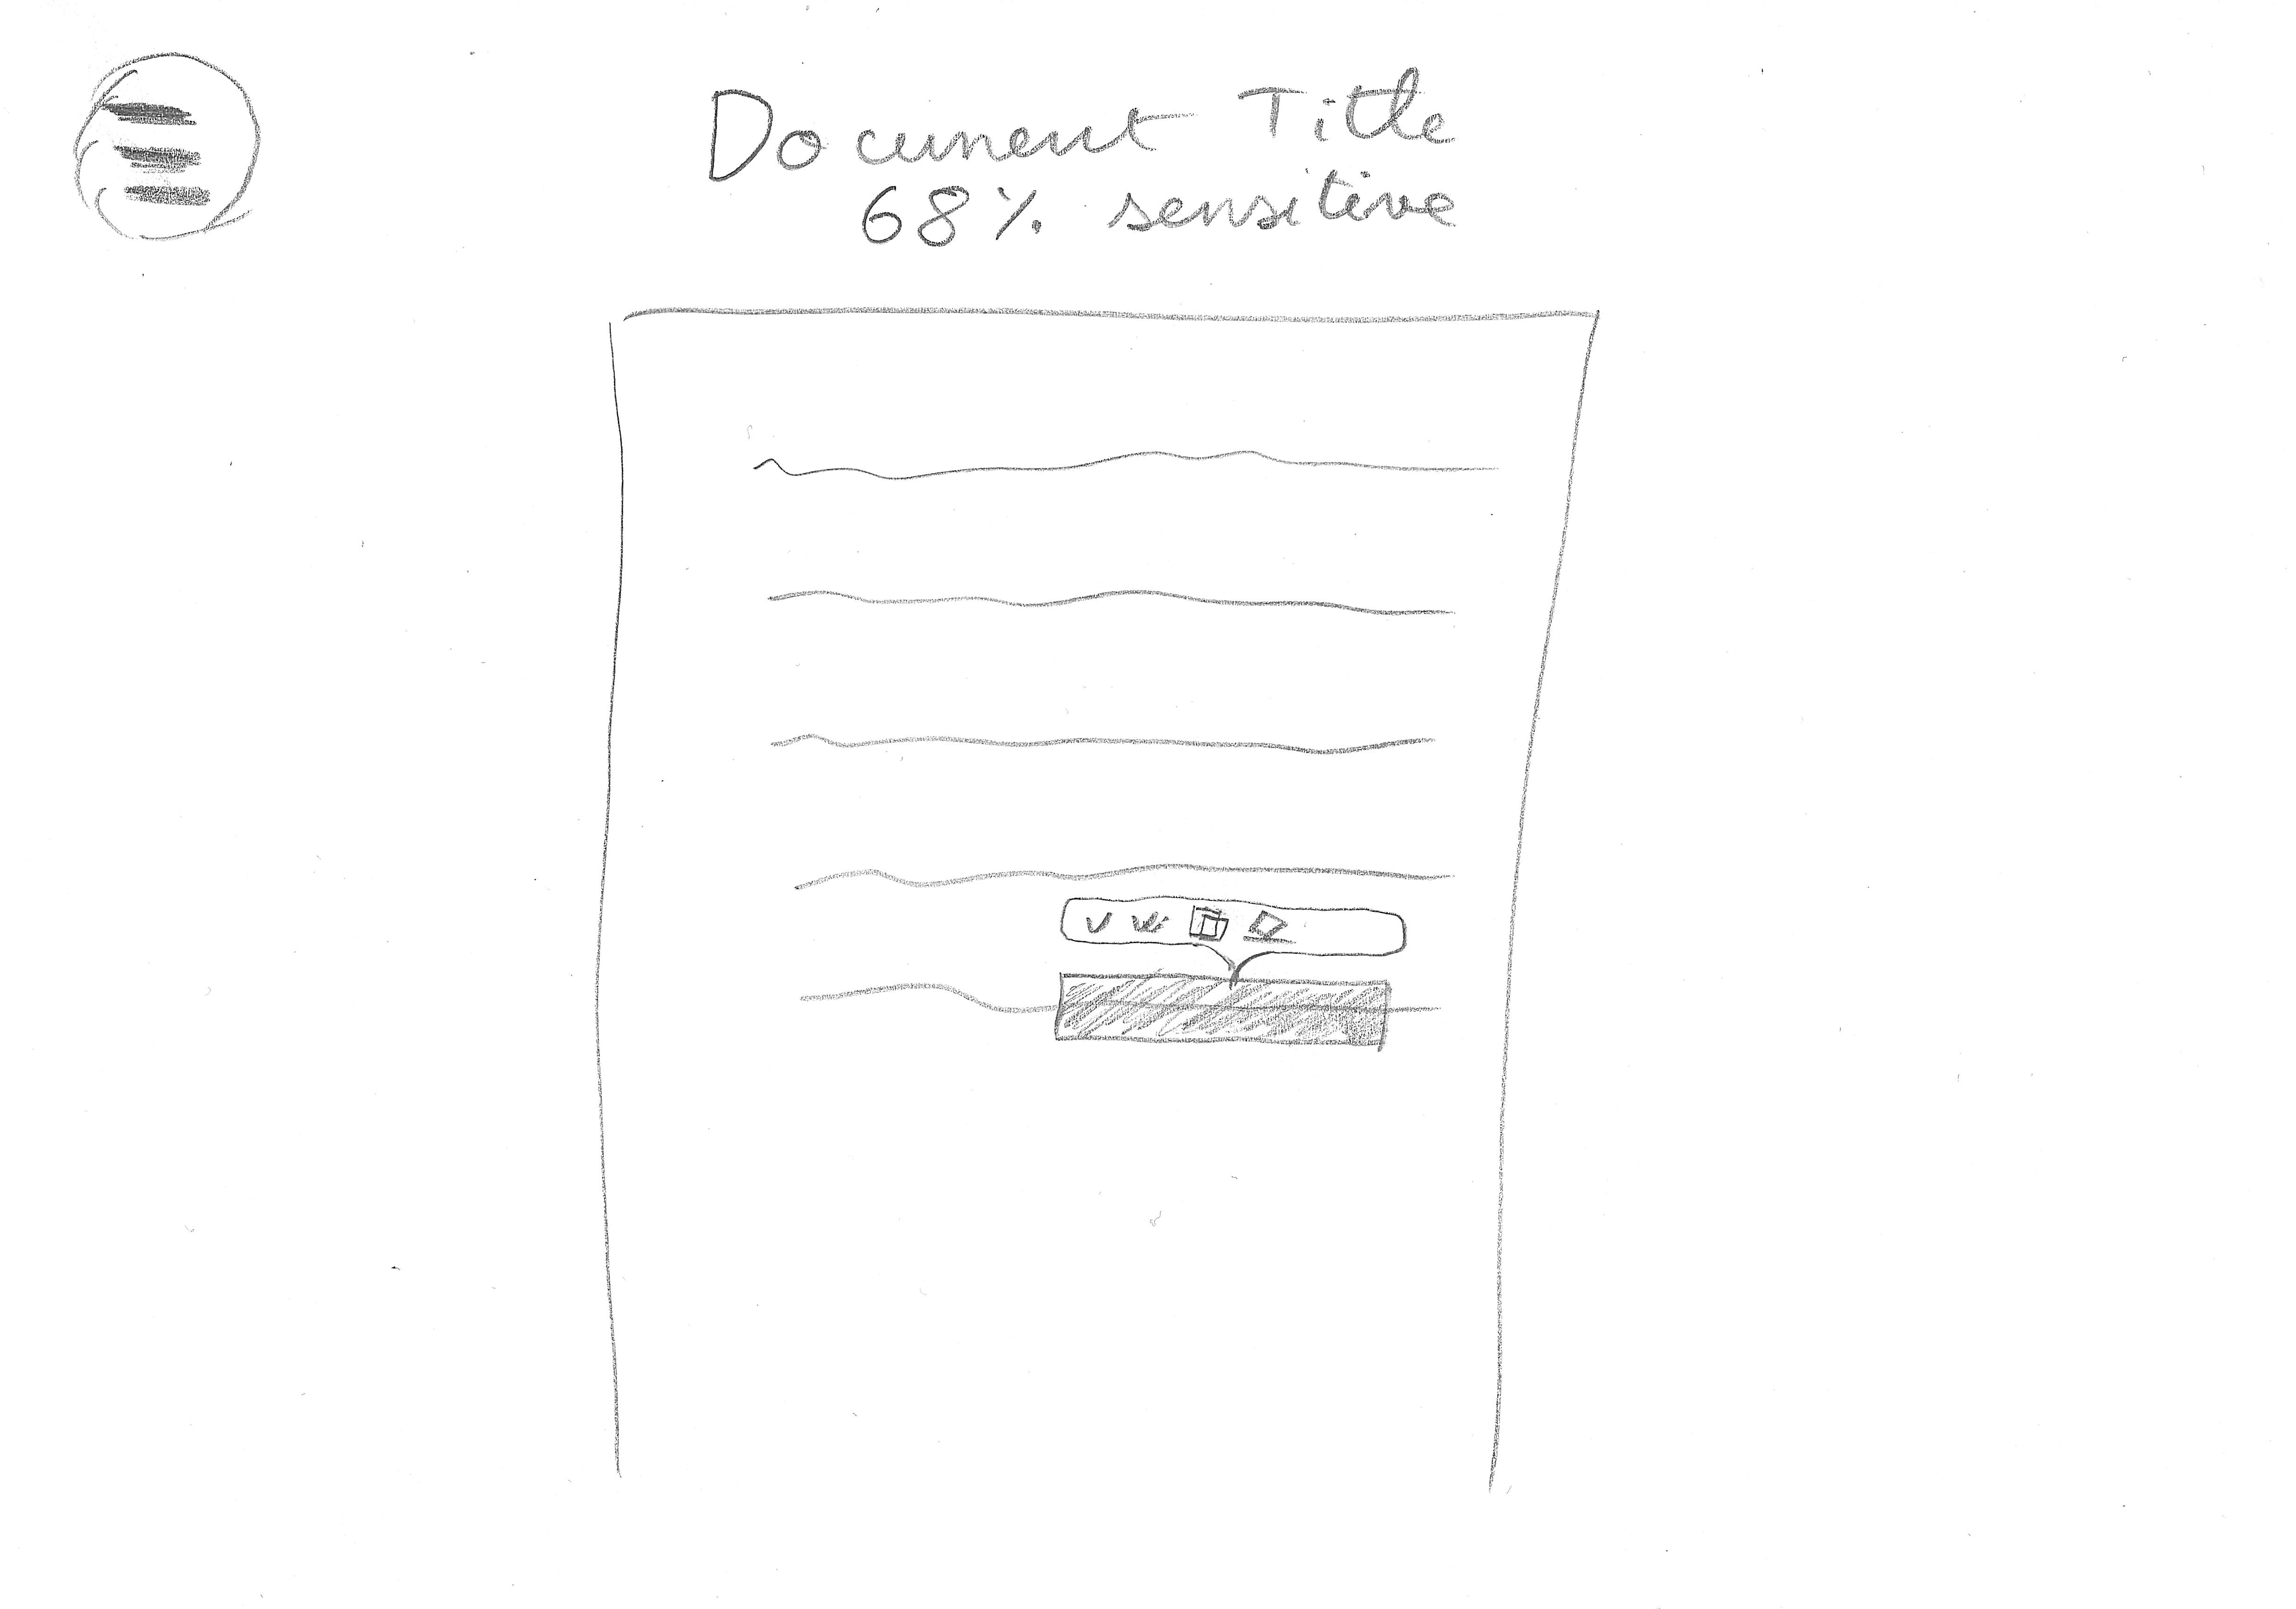
\includegraphics[width=\linewidth]{images/wireframes/page.png}
    \end{figure}
    \section{Document View v2 - opened settings drawer}
    \begin{figure}[H]
        \centering
        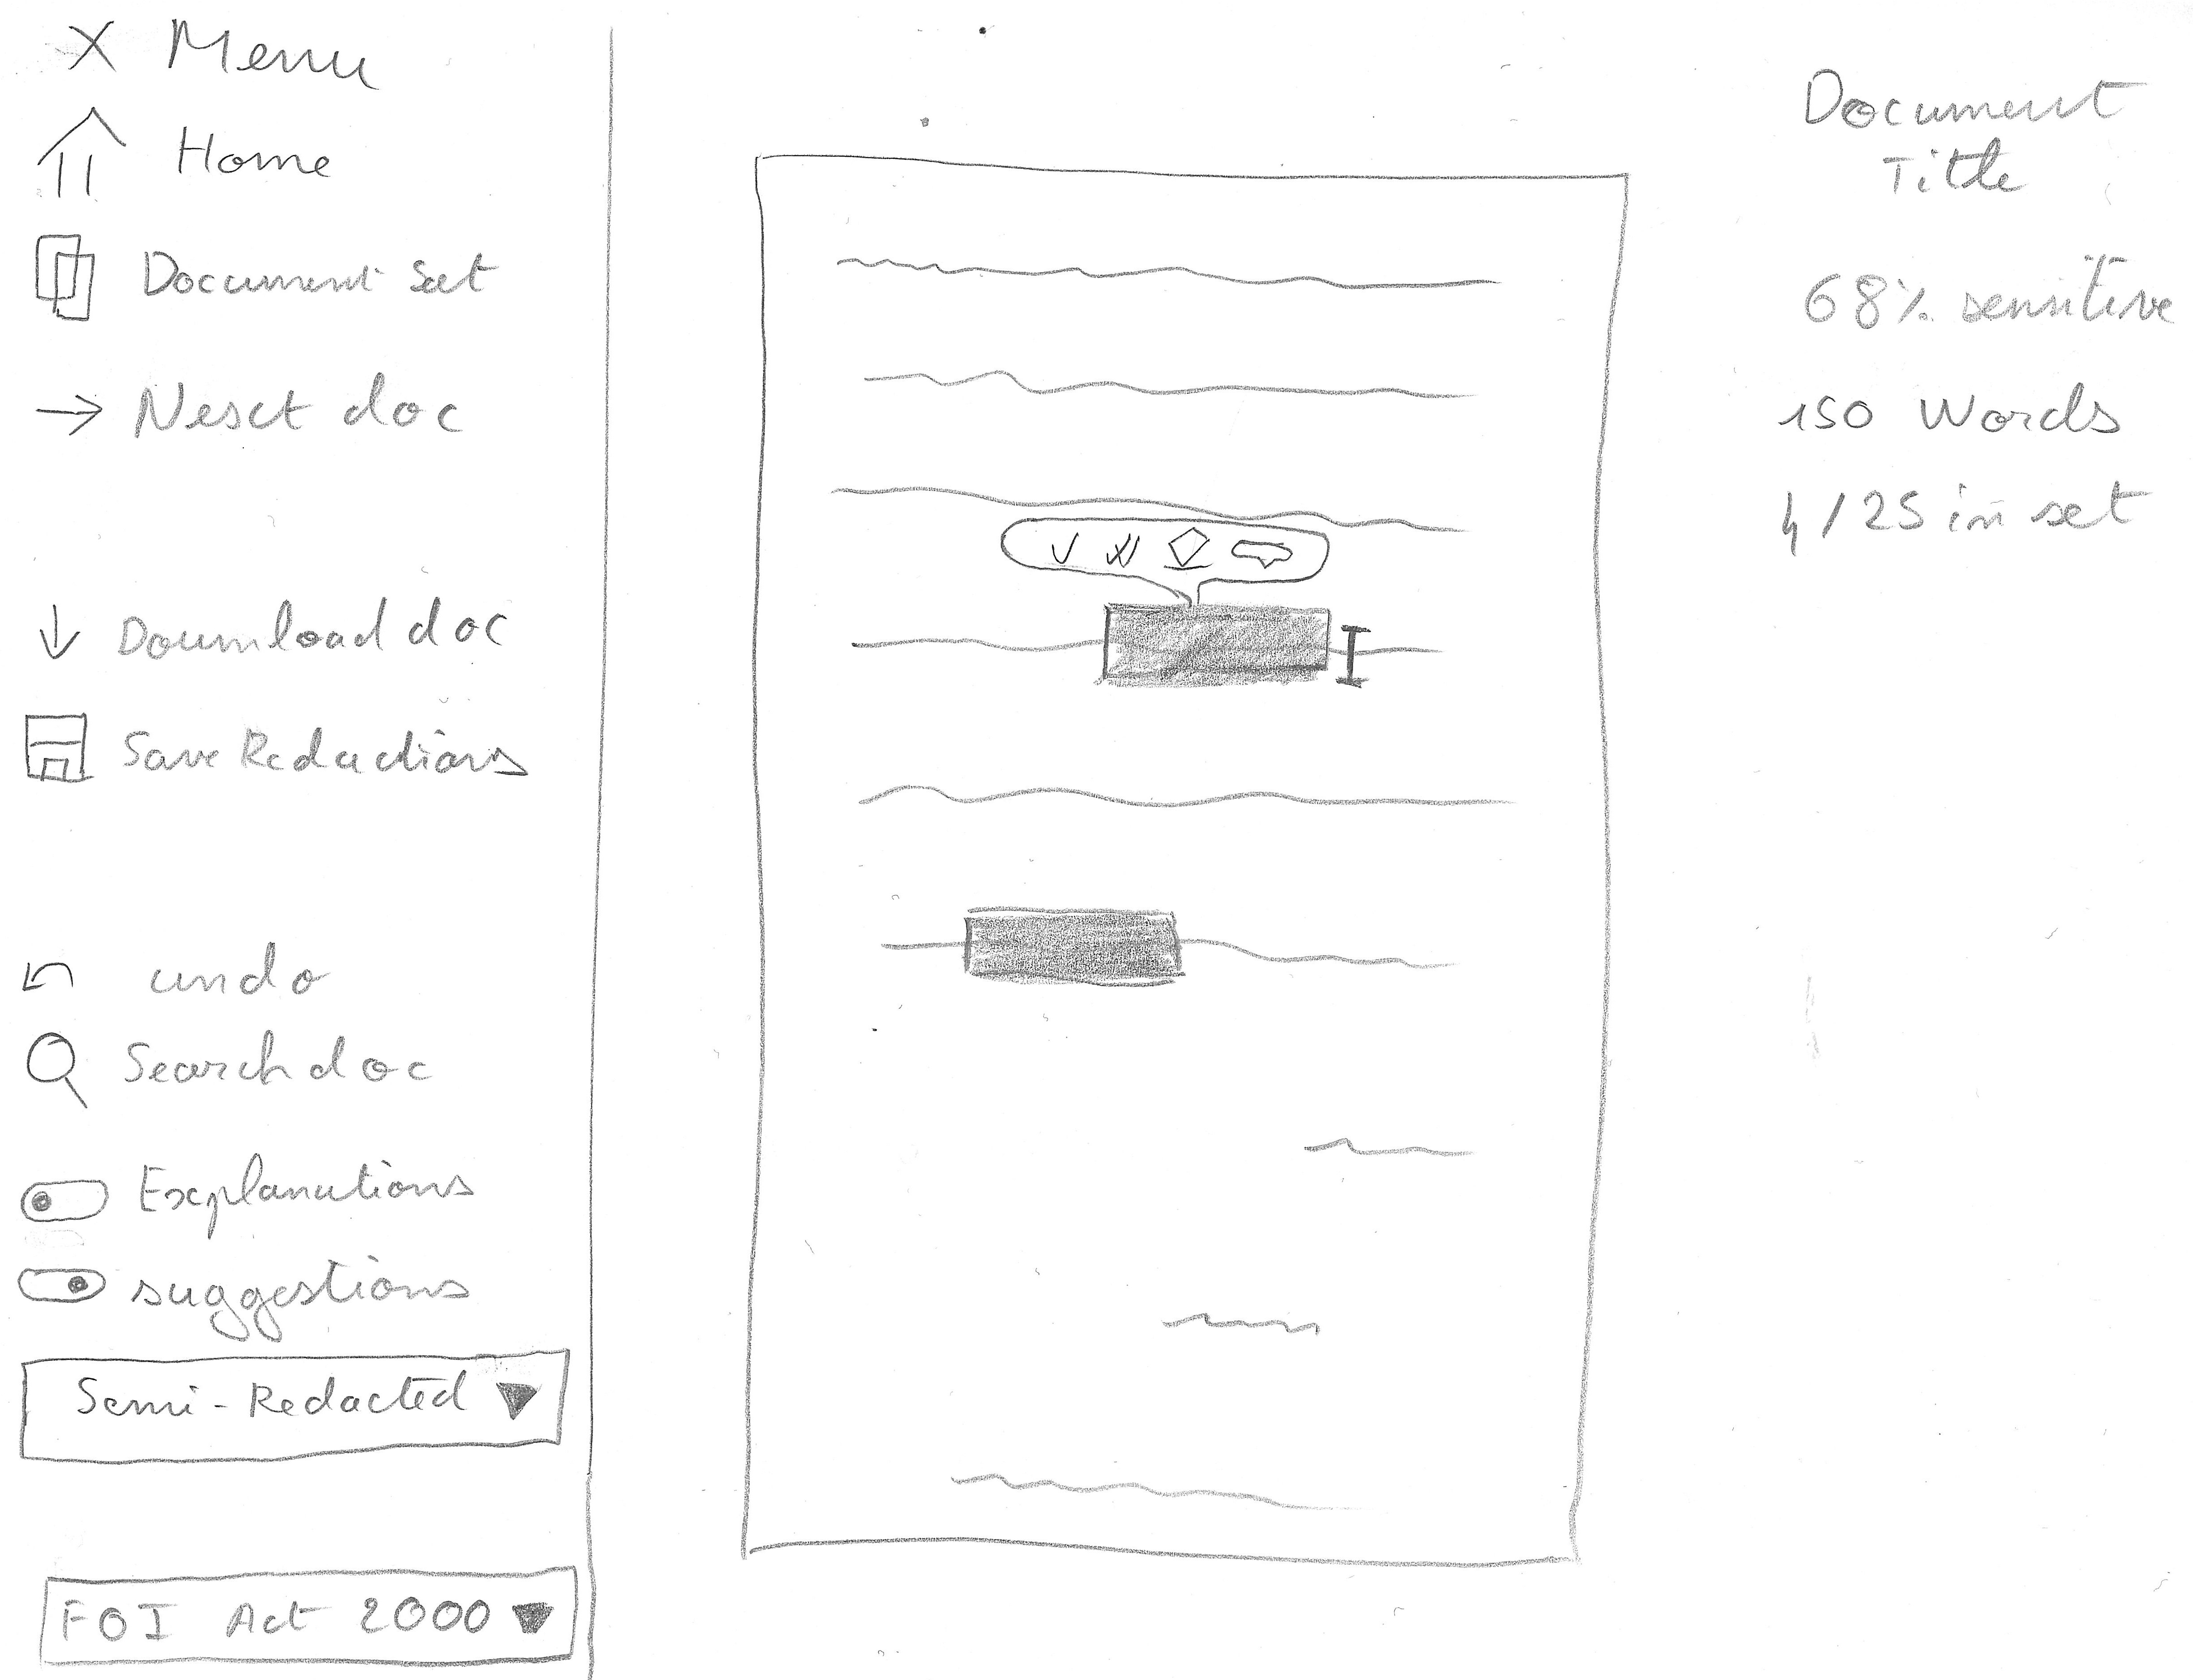
\includegraphics[width=\linewidth]{images/wireframes/doc_view.jpg}
    \end{figure}
    \section{Document View v2 - closed settings drawer}
    \begin{figure}[H]
        \centering
        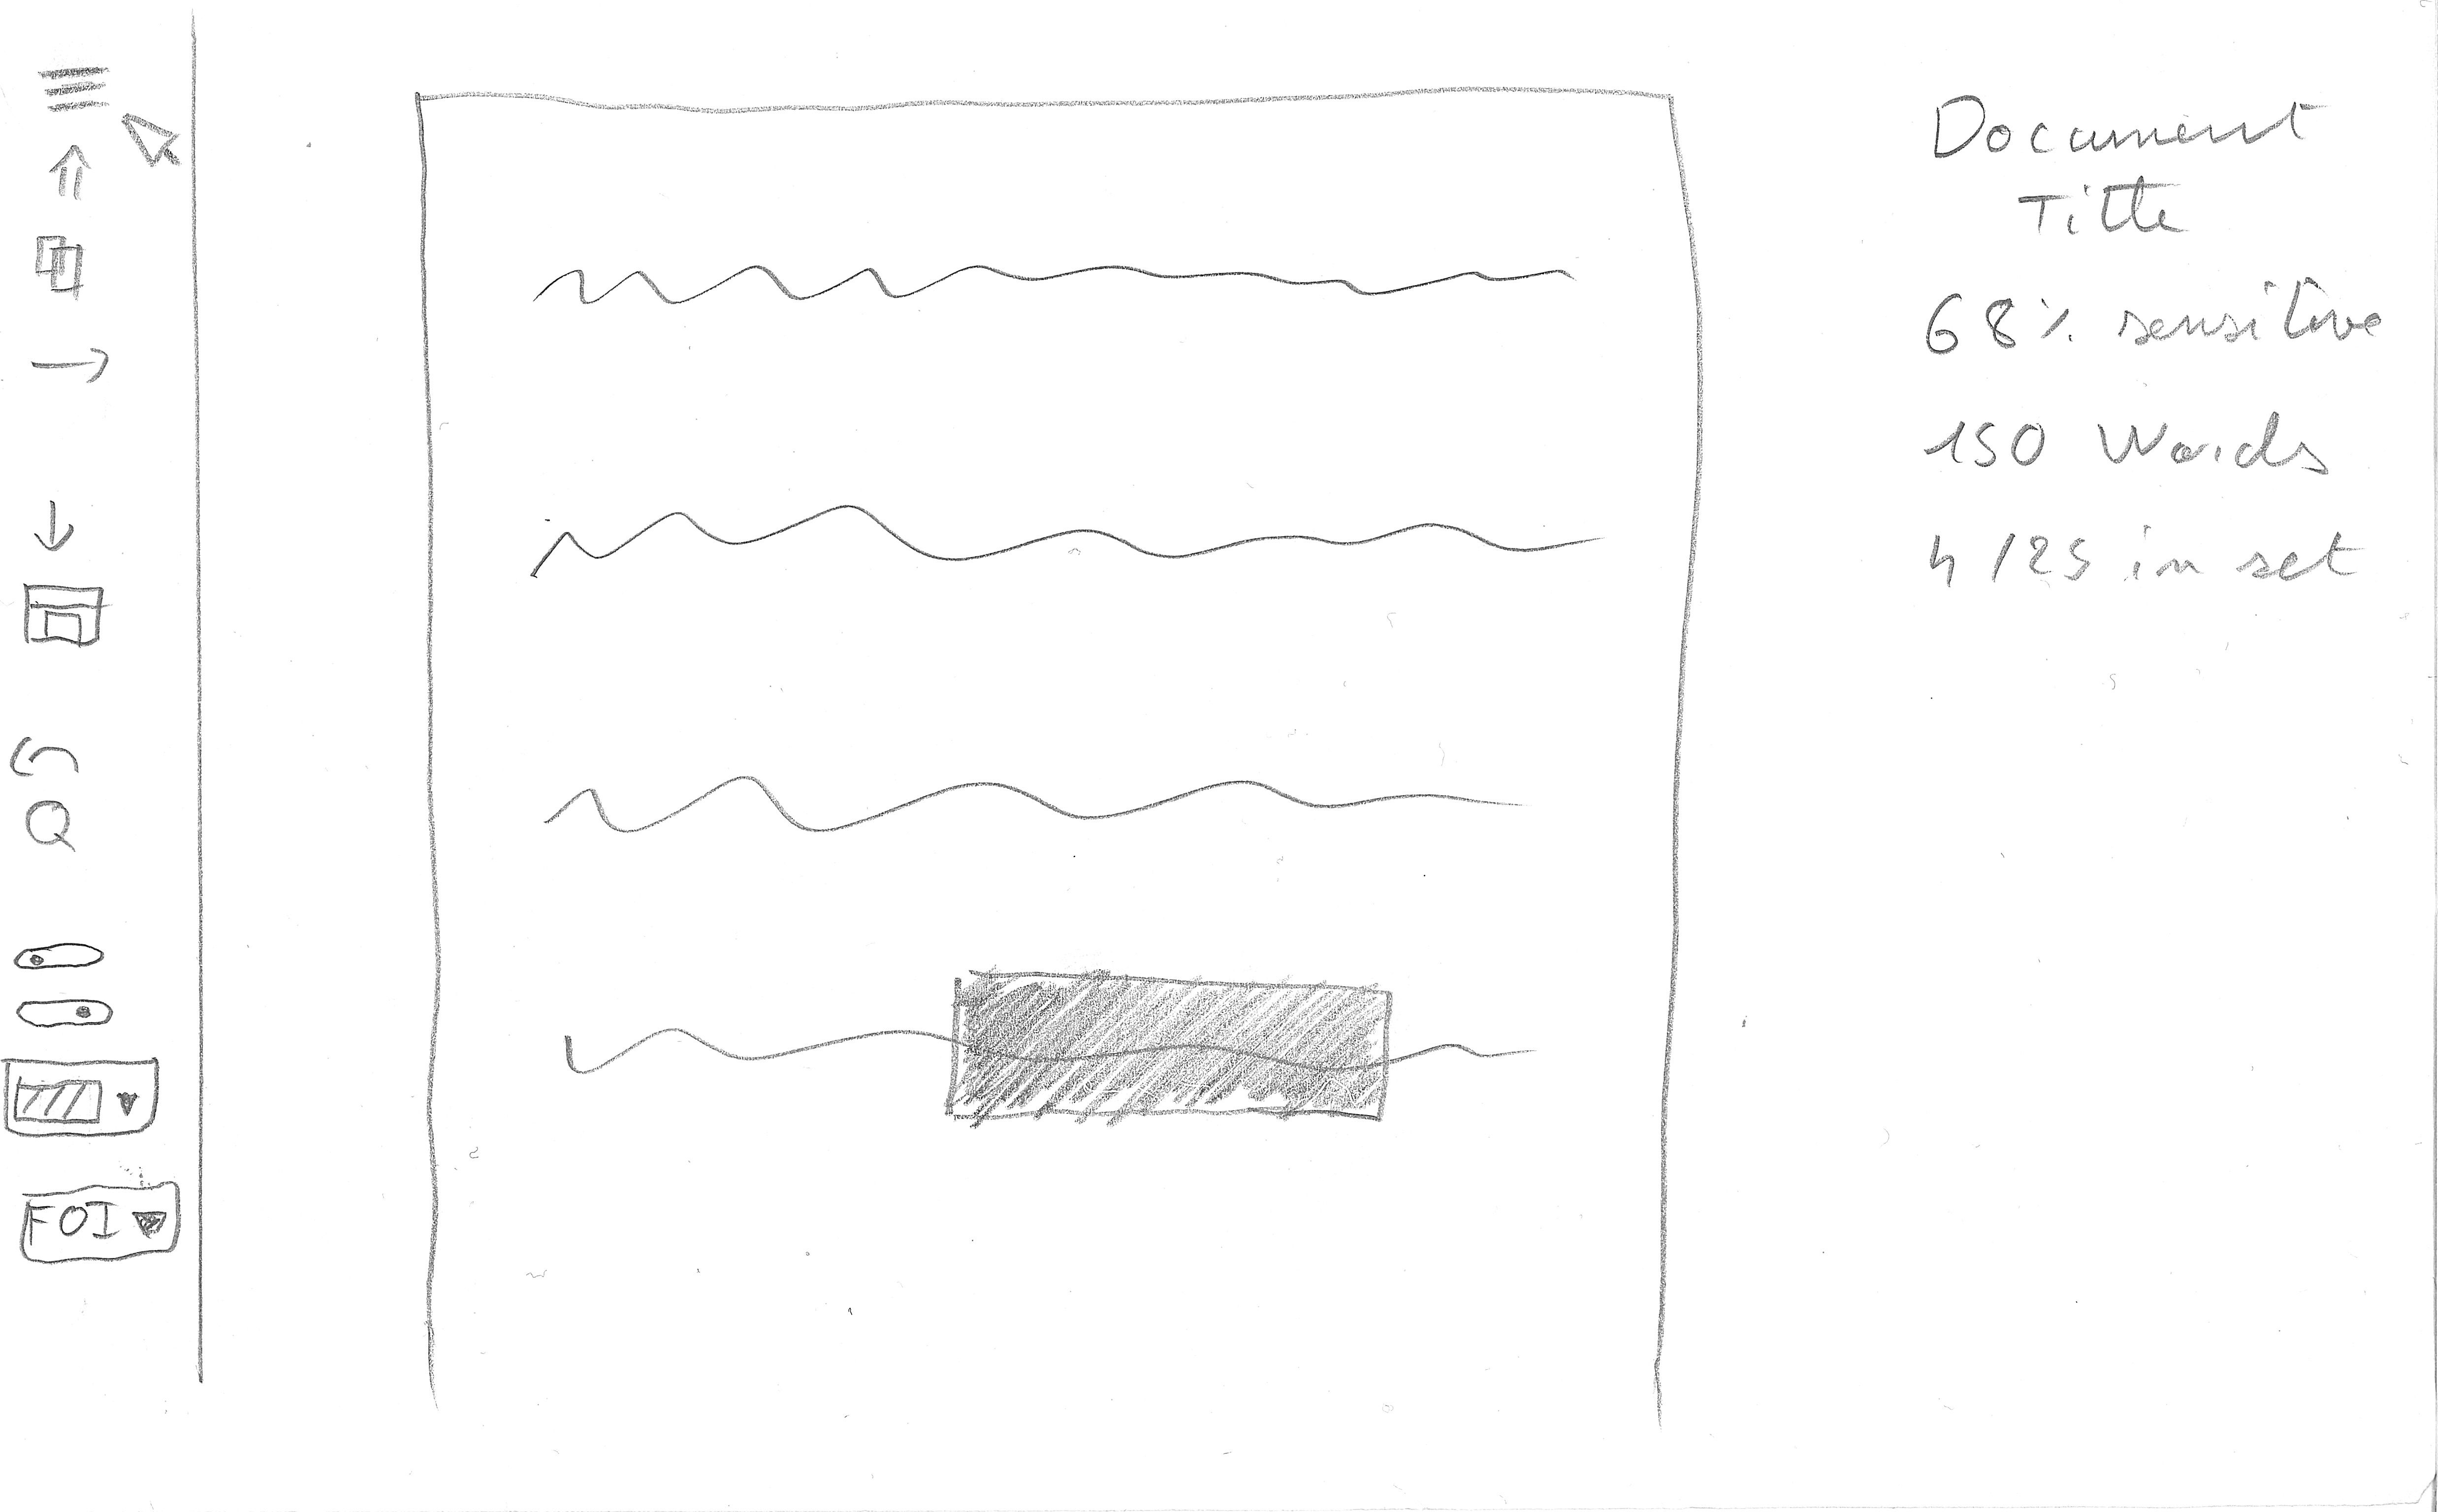
\includegraphics[width=\linewidth]{images/wireframes/doc-view.jpg}
    \end{figure}
    \section{Text Select Tooltip}
    \begin{figure}[H]
        \centering
        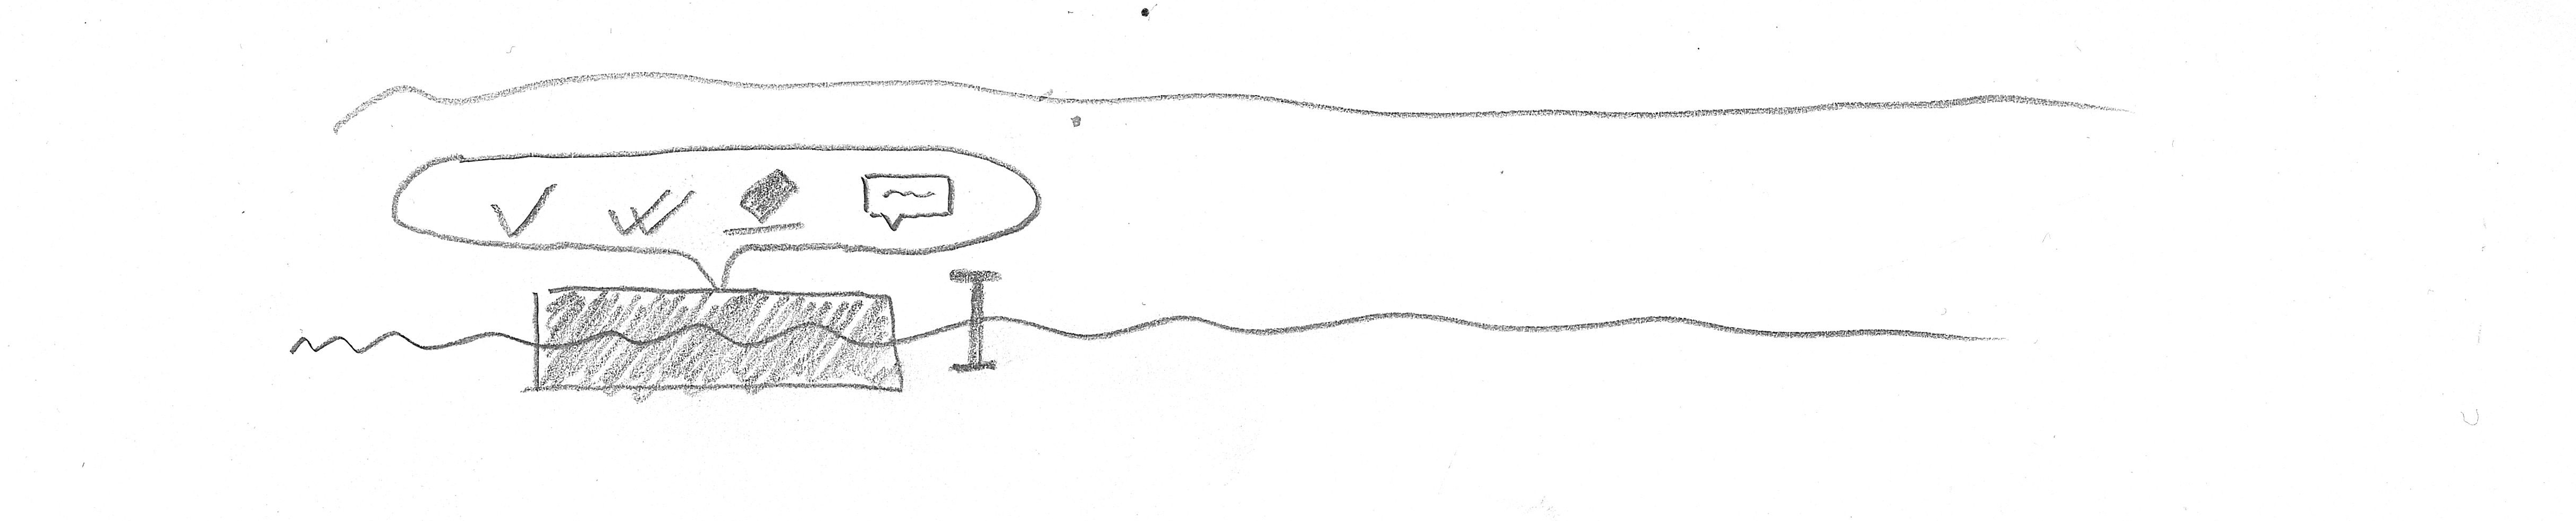
\includegraphics[width=\linewidth]{images/wireframes/tooltip.jpg}
    \end{figure}
    \section{Text Select Tooltip - opened comment menu}
    \begin{figure}[H]
        \centering
        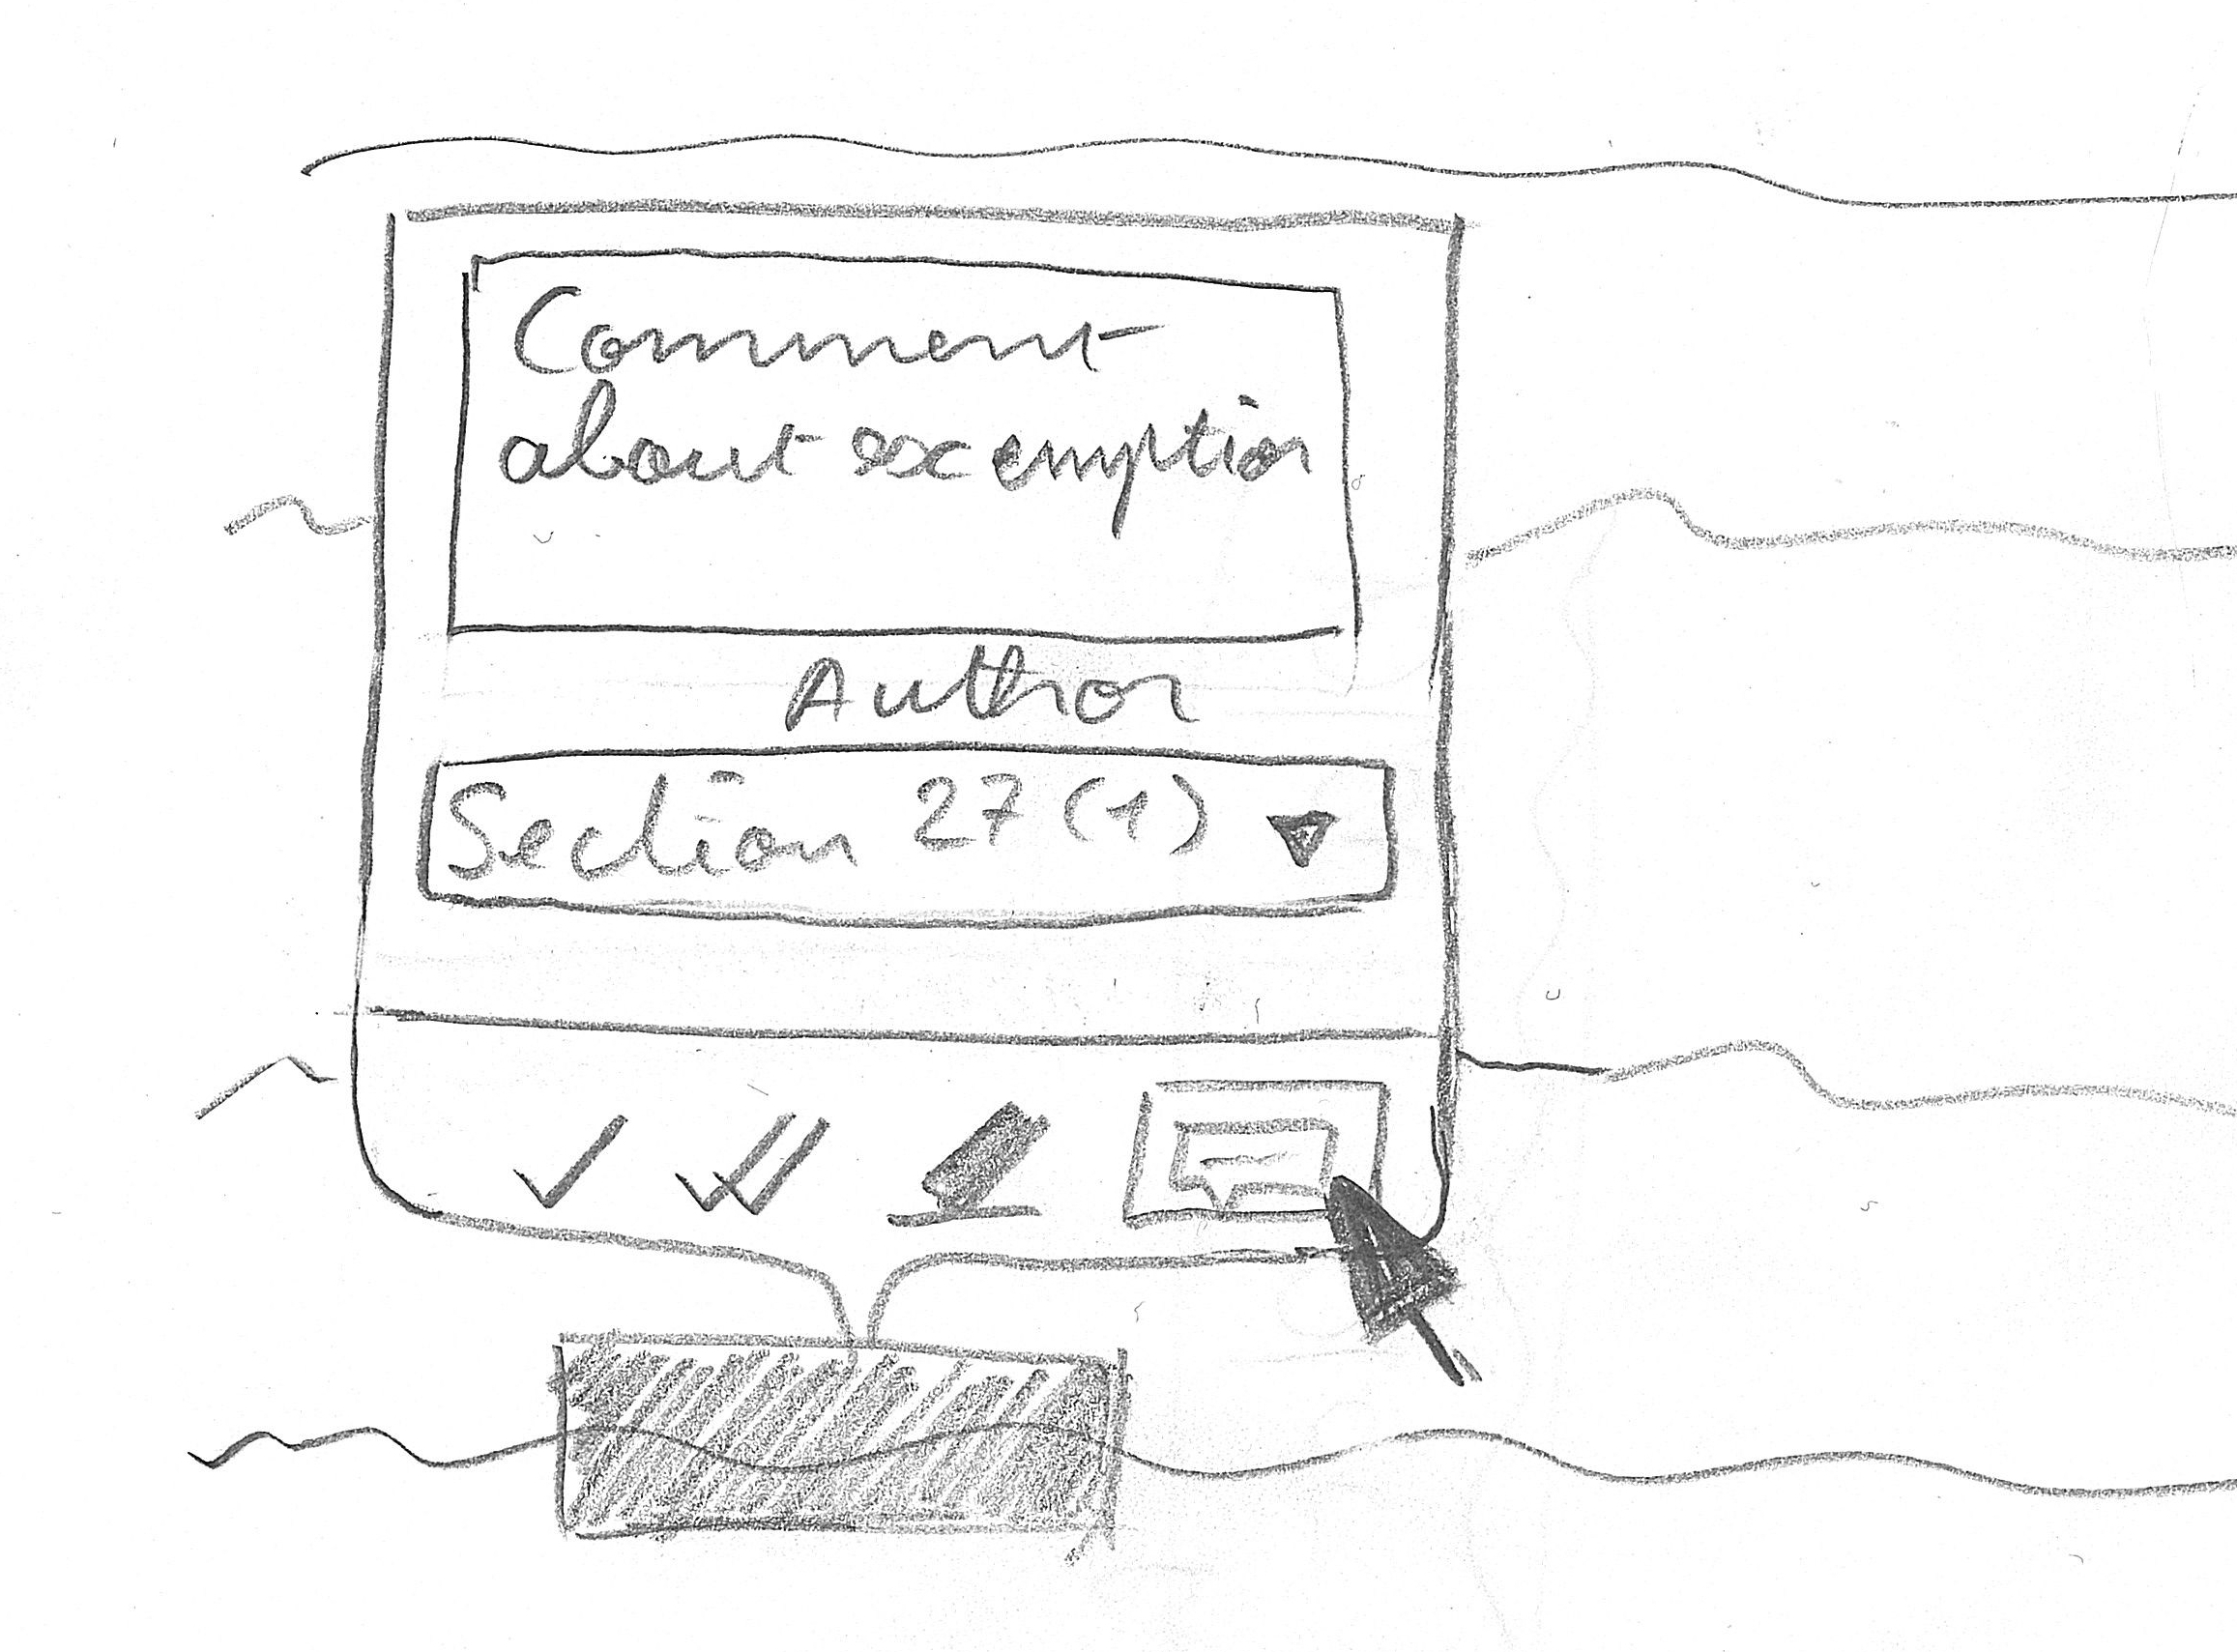
\includegraphics[width=\linewidth]{images/wireframes/tooltip_comment.jpg}
    \end{figure}
    \chapter{User evaluation questionnaire}\label{appendix:questionnaire}
    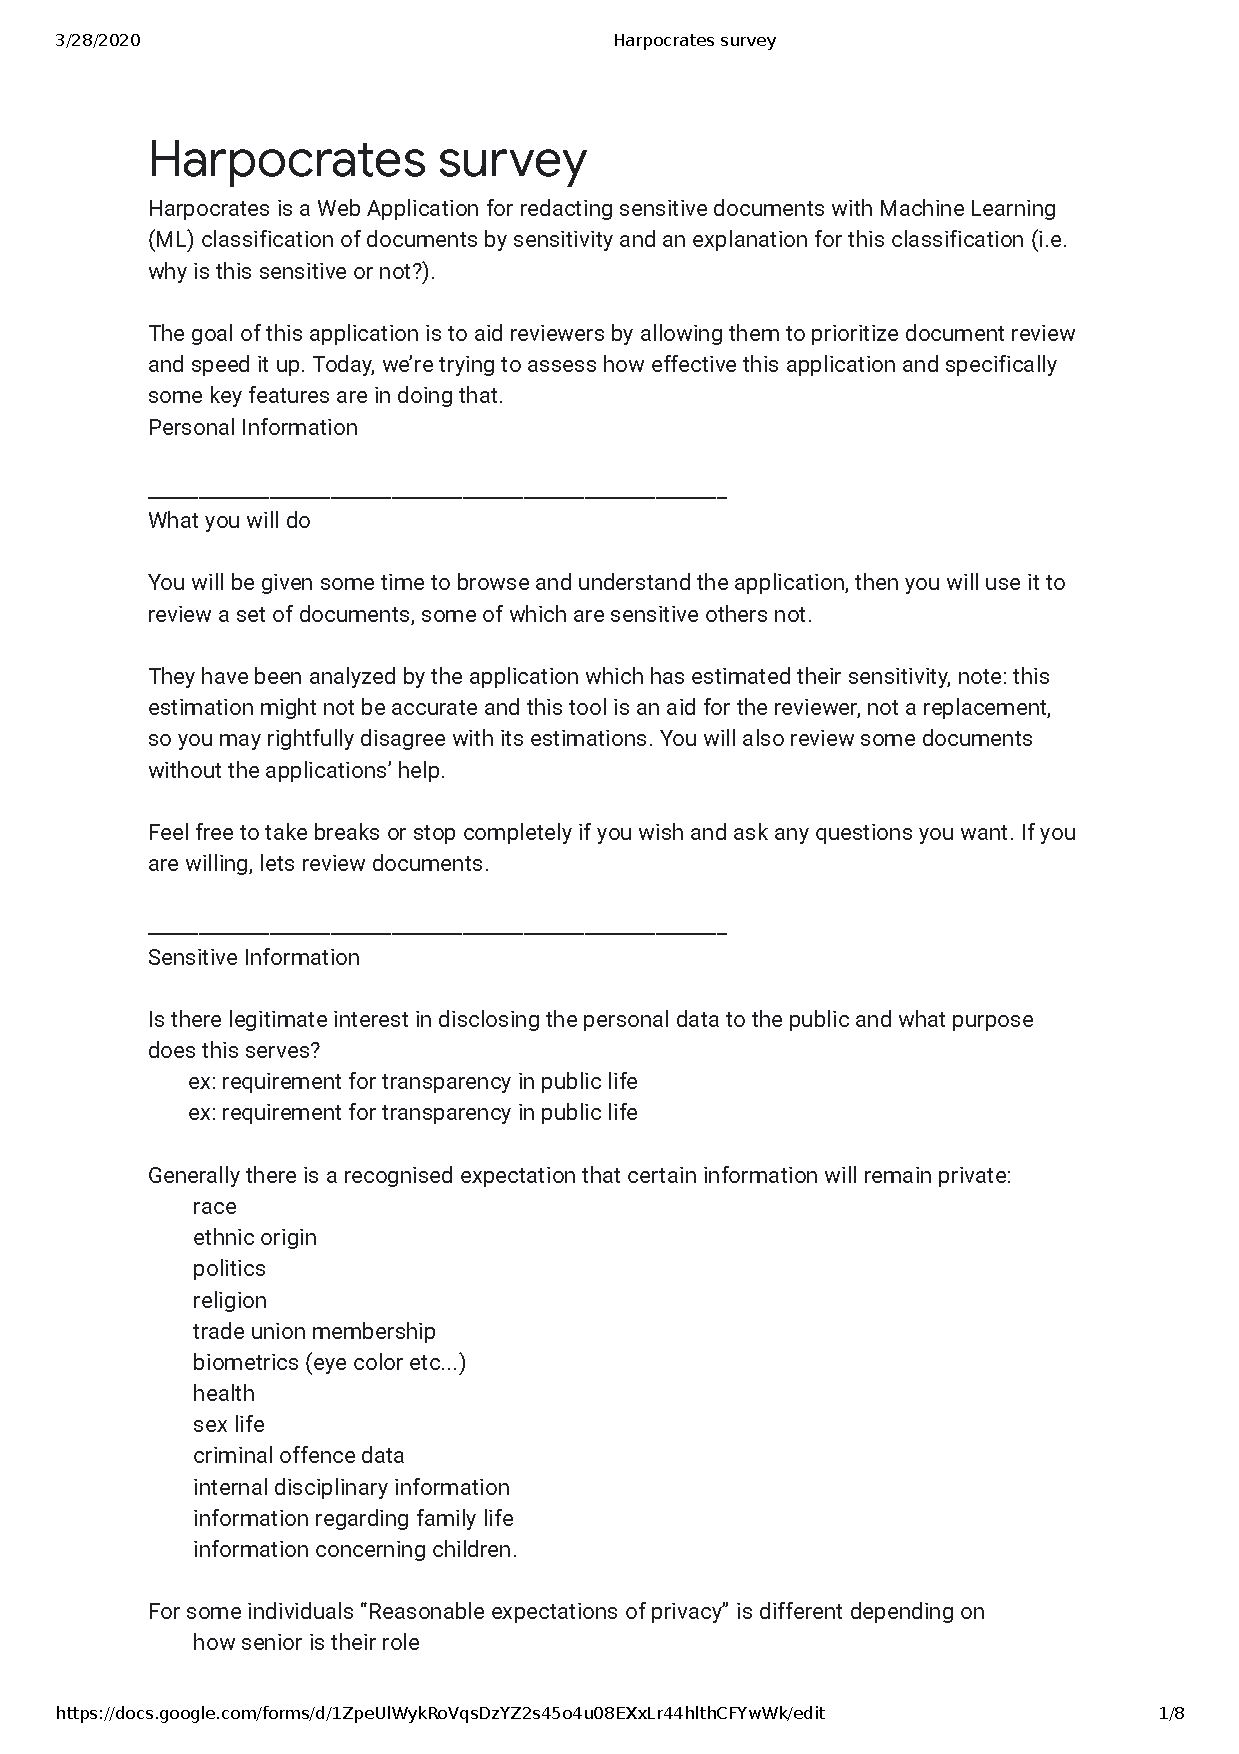
\includepdf[
        pages=-,
        % pagecommand={},
        % width=\linewidth
    ]{figures/questionnaire.pdf}
\end{appendices}
%==================================================================================================================================
%   BIBLIOGRAPHY   


\newpage


\section*{References}

\printbibliography[heading=none]

\vspace*{\fill}
% print license
\doclicenseThis%

\end{document}